% !TeX root = main.tex

\documentclass[10pt,aspectratio=169,dvipsnames]{beamer} % sets document type, default font size, slide aspect ratio, and loads color names
\usetheme[color/block=transparent]{metropolis} % sets the theme of the document

\usepackage[absolute,overlay]{textpos} % allows absolute positioning of text
\usepackage{booktabs} % enhances quality of tables
\usepackage[utf8]{inputenc} % allows input encoding in UTF-8
\usepackage{tikz} % used for creating vector graphics
\usetikzlibrary{arrows.meta} % loads additional arrow types
\usepackage[europeanresistors,americaninductors]{circuitikz} % for drawing electrical circuits
\usepackage[scale=2]{ccicons} % loads Creative Commons icons
\usepackage[official]{eurosym} % loads the official symbol for the Euro
\usepackage{hyperref} % allows creating hyperlinks in the document

\newcommand{\ra}[1]{\renewcommand{\arraystretch}{#1}} % creates command to adjust spacing between rows
\newcommand{\hrefc}[2]{\href{#1}{\bf\color{blue}{\underline{#2}}}} % defines command for underlined, blue hyperlink
\newcommand{\urlc}[1]{\hrefc{#1}{#1}} % defines command for URL hyperlink

\newcommand{\R}{\mathbb{R}} % creates a shortcut for typing real numbers symbol
\newcommand{\ubar}[1]{\text{\b{$#1$}}} % defines a command for underlined text

\xdefinecolor{TUred}{RGB}{197,14,31} % defines a new color TUred
\setbeamerfont{alerted text}{series=\bfseries} % sets the font of alerted text to bold
\setbeamercolor{alerted text}{fg=TUred} % sets the color of alerted text to TUred
\setbeamercolor{background canvas}{bg=white} % sets the background color to white
\setbeamercolor{frametitle}{bg=lightgray!40, fg=TUred} % sets the background color of the frame title to light gray and text color to TUred
\setbeamercolor{title}{fg=TUred} % sets the color of the title to TUred

\addtobeamertemplate{frametitle}{}{% adds image to every frame title
  \begin{textblock*}{100mm}(1.01\textwidth,2pt)
    
\includegraphics[width=1.5cm]{images/TUB.png}
    \end{textblock*}}

\def\l{\lambda} % defines a shortcut for lambda symbol
\def\m{\mu} % defines a shortcut for mu symbol
\def\d{\partial} % defines a shortcut for partial symbol
\def\cL{\mathcal{L}} % defines a shortcut for caligraphic L symbol
\def\co{CO${}_2$} % defines a shortcut for CO2 symbol
\def\el{${}_{el}$} % defines a subscript for el
\def\th{${}_{th}$} % defines a subscript for th
\def\gas{${}_{gas}$} % defines a subscript for gas

\setbeamercolor{framesource}{fg=gray} % sets color of framesource to gray
\setbeamerfont{framesource}{size=\tiny} % sets font size of framesource to tiny
\newcommand{\source}[1]{% creates command for inserting a source footnote
\begin{textblock*}{5cm}(10.5cm,8.35cm)
    \begin{beamercolorbox}[ht=0.5cm,right]{framesource}
        \usebeamerfont{framesource}\usebeamercolor[fg]{framesource} {#1}
    \end{beamercolorbox}
\end{textblock*}}

\graphicspath{{../results/}} % sets the path where graphics can be found
\DeclareGraphicsExtensions{.pdf,.jpeg,.png,.jpg} % defines the types of graphic files that can be used

\def\goat#1{{\scriptsize\color{green}{[#1]}}} % defines a command for green, scriptsize text

\let\olditem\item % saves the old item command
\renewcommand{\item}{\olditem\vspace{5pt}} % redefines the item command to add space after each item


\title{On space-time load-shifting flexibility for data centers \\ 
      \& 24/7 carbon-free electricity procurement}

%\subtitle{---}
\author{
  Iegor Riepin, Tom Brown\\
  \hrefc{https://www.tu.berlin/en/ensys}{Department of Digital Transformation in Energy Systems}, TU Berlin
  }

\date{30 June 2023}

\titlegraphic{%
  \vspace{0cm}
  \hspace{10.7cm}
    
\includegraphics[trim=0 0cm 0 0cm,height=1.2cm,clip=true]{images/TUB.png}
  \vspace{5.5cm}
  \\ \faGithub \href{https://github.com/PyPSA/247-cfe}{ Code to reproduce this study}
  }

\begin{document}

\maketitle

\begin{frame}
  \frametitle{Acknowledgements}

  \begin{itemize}
    \item {\bf Funding:} This study was supported by a grant from Google, Inc. 
    \item {\bf Acknowledgements:} The authors thank members of the Google energy markets and policy team 
    for their feedback and inputs on earlier drafts of this study. 
    We also thank the \hrefc{https://pypsa.org/}{PyPSA team} and many contributors to the open-source 
    energy system modelling ecosystem used for this study (see: \hrefc{https://github.com/PyPSA/PyPSA}{github.com/PyPSA}).
    Warm thanks to Fabian~Hofmann for making complex optimization simpler with \hrefc{https://linopy.readthedocs.io/}{linopy}. 
    \item 
    {\bf Copyright} Unless otherwise stated, graphics and text are Copyright \copyright Tom Brown and Iegor Riepin, 2023.
    Graphics and text for which no other attribution are given are licensed under a 
    \href{https://creativecommons.org/licenses/by/4.0/}{CC BY 4.0}.  {\footnotesize \ccby} 
    \item The content of this study, including any errors or omissions, are the responsibility
    of the authors alone.
  \end{itemize}

\end{frame}


\begin{frame}{Summary of key findings TODO}

  \centering
  {\small

  \noindent\fbox{%
  \parbox{\textwidth}{%
    \begin{enumerate}

    % \item 24/7~carbon-free energy (CFE) procurement leads to lower emissions for both the buyer and the system,
    %   as well as reducing the needs for flexibility in the rest of the system.  

    % \item Reaching CFE for 90-95\% of the time can be done with only a small cost premium compared to annually matching 
    % 100\% renewable energy. 90-95\% CFE can be met by supplementing wind and solar with battery storage.

    % \item Reaching 100\% CFE target is possible but costly with existing renewable 
    % and storage technologies, with costs increasing rapidly above 95\%.
    
    % \item 100\% CFE target could have a much smaller cost premium if long duration storage or 
    % clean dispatchable technologies like advanced geothermal are available.
    
    % \item 24/7~CFE procurement would create an early market for the advanced technologies,
    % stimulating innovation and learning from which the whole electricity system would benefit.
    
    \item Space-time load-shifting flexibility facilitates economically efficient redistribution of data center loads.
    \item This effect comes with a ... and reduction of renewable energy curtailment.
    \item Flexible operation helps achieving a 24/7 hourly matching of electricity demand with clean energy with smaller resources. This can facilitate more data center operators and other flexible electricity buyers to join the 24/7~CFE efforts. 
    \item Space-time load management can enable achieving 24/7~CFE procurement goals simpler for other companies who do not have such flexibility options. 
    \item on LDES? on emission reduction with lower cost?

  \end{enumerate}
  }}
  }
  
\end{frame}



\begin{frame}
  \frametitle{Table of Contents}
  \setbeamertemplate{section in toc}[sections numbered]
  \tableofcontents[hideallsubsections]
\end{frame}


%----------------------------------------
%----------------------------------------

\section{Introduction}


\begin{frame}{Introduction}

  {\footnotesize
  \centering
  \begin{columns}[T]
  \begin{column}{9cm}
    \begin{itemize}
    \item Climate change is driving a global effort to \alert{rapidly decarbonise} 
    electricity systems across the globe. Many public and private energy buyers join this effort. For example, more than 380 members of the \hrefc{https://www.there100.org/}{RE100 group} have committed to procure enough renewable energy to match 100\% of their electricity consumption on an annual basis.

    \item Fully decarbonizing electricity grids, however, requires generating carbon-free energy when it is needed, not just during periods of abundant sunshine or wind. This challenge requires embracing \hrefc{https://www.iea.org/reports/advancing-decarbonisation-through-clean-electricity-procurement}{innovative strategies} for decarbonization. 
    There is growing interest from leaders in voluntary clean  electricity procurement to cover their consumption with clean energy supply on a \alert{truly 24/7 basis}.  Achieving 24/7 Carbon-Free Energy (CFE) means that every kilowatt-hour of electricity consumption is met
    with carbon-free electricity sources around-the-clock.

    \item The \hrefc{https://www.un.org/en/energy-compacts/page/compact-247-carbon-free-energy}{24/7 Carbon-Free Energy Compact}, coordinated by the United Nations now includes more than 120 signatories on a mission to realize a 24/7 Carbon-Free Energy future. 

    \end{itemize}
    \end{column}

    \begin{column}{6cm}
    \centering
    \vspace{0.3cm}
    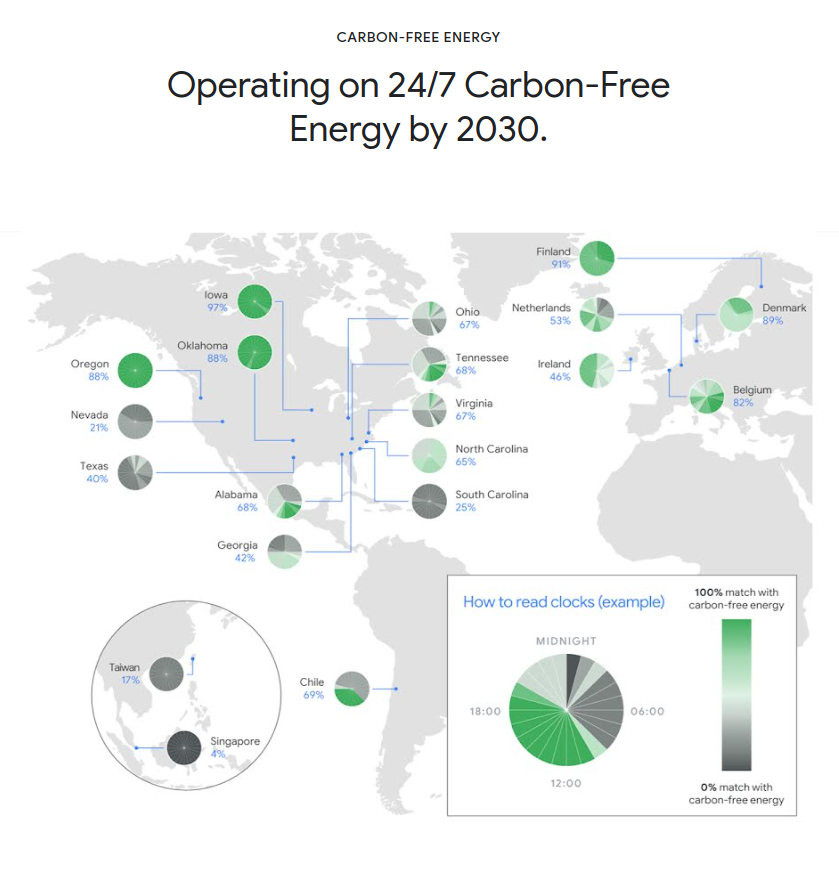
\includegraphics[width=6cm]{images/247-google-web.png}
    \vspace{.1cm}
  \end{column}

  \source{\href{https://sustainability.google/progress/energy/}{Image: sustainability.google/progress/energy/}}
  \end{columns}

  }
\end{frame}


\begin{frame}{Introduction}

  {\footnotesize
  \begin{itemize}
  \item In October 2022, we published a study on the \hrefc{https://zenodo.org/record/7180097}{"System-level impacts of 24/7 carbon-free electricity procurement in Europe"} \\
  \faGithub~\hrefc{https://github.com/PyPSA/247-cfe/releases/tag/v0.1}{Code behind the study}. 
  
  \item In this study, we investigated the \alert{means and costs} of pursuing different clean electricity procurement strategies for companies in a selection of European countries. We also explored how the 24/7~CFE commitments \alert{affect the European electricity system} as a whole. 
  
  \item The study concluded that 24/7~CFE procurement has the following impacts: \\ 
  (i) lower emissions for both the participating consumers and within the background electricity grids;\\ 
  (ii) reduction of the needs for flexibility in the rest of the system; \\ 
  (iii) increase in energy costs for participating consumers for CFE targets above 95\% (which could be significantly reduced if long duration energy storage or clean firm generation technologies are available); \\ 
  (iv) stimulating innovation and learning, and creation of an early market for the advanced technologies.

  \item  These European study results align with the results in studies done by \hrefc{https://acee.princeton.edu/24-7/}{Princeton ZERO lab (2021)} for regions in the United States and by \hrefc{https://www.iea.org/reports/advancing-decarbonisation-through-clean-electricity-procurement}{IEA (2022)} for regions in Asia and Indonesia.

  \end{itemize}
  }

\end{frame}
  


\begin{frame}{Motivations}

  {\footnotesize
  \begin{itemize}
  \item In the previous study, however, we focused on a large range of European companies from the commertial and industry (C\&I) sectors that join 24/7~CFE efforts in aggregate. The implicit assumption we made was that all 24/7~CFE participants have an \alert{inflexible demand}.
  
  \item In reality, many particiapnts of the 24/7~CFE movement have some degree of flexibility in their electricity consumption. The flexibility takes form of various demand response mechanisms available for \hrefc{https://doi.org/10.1016/j.rser.2021.111963}{a wide range} of commertial and industry consumers.

  \item  A \hrefc{https://cerre.eu/publications/data-centres-and-the-energy-grid}{large potential for demand side flexiblity} is created by the information and communications technology (ICT) sector. Big companies such as Amazon, Google, IBM, and Microsoft are centralizing data centers to achieve economies of scale and form a computing infrastructure that is managed collectively via network operation centers. Thus, data center operators have the ability to \alert{shift computing jobs and associated power loads} in time (via scheduling of flexible compute jobs) and in space (via migration of flexible compute jobs across locations). 
  \end{itemize}

  }

\end{frame}
  

\begin{frame}{Why is this important? 1/2}

  {\footnotesize

  \begin{columns}[T]
    \begin{column}{9cm}
      \begin{itemize}
        \item   
        Demand for computing resources and data center power is rapidly growing, now representing nearly \hrefc{https://doi.org/10.1126/science.aba3758}{1\% of final electricity demand} worldwide. 
        Data centres and data transmission networks are responsible for \hrefc{https://www.iea.org/reports/data-centres-and-data-transmission-networks}{0.9\% of energy-related GHG emissions} (around 300~Mt \co-eq in 2020).
      
        \item Despite rapidly growing demand for digital services, the growth of associated emissions was modest due to energy efficiency improvements, decarbonisation of electricity grids and renewable energy purchases by ICT companies above and beyond the policy obligations. Based on \hrefc{https://www.iea.org/reports/data-centres-and-data-transmission-networks}{IEA (2022)} estimates, Amazon, Microsoft, Meta and Google have become the four largest purchasers of corporate renewable energy, having contracted over 38~GW to date with power purchase agreements (PPAs).
      
        \item Moreover, some of the ICT companies have become the front runners of the 24/7~CFE movement. Google has committed to the goal of \hrefc{https://www.gstatic.com/gumdrop/sustainability/247-carbon-free-energy.pdf}{24/7 Carbon-Free Energy by 2030}. Similarly, Microsoft has announced own \hrefc{https://blogs.microsoft.com/blog/2021/07/14/made-to-measure-sustainability-commitment-progress-and-updates/}{100/100/0 by 2030} commitment.

      \end{itemize}
      \end{column}
  
      \begin{column}{6cm}
      \centering
      \vspace{.3cm}
      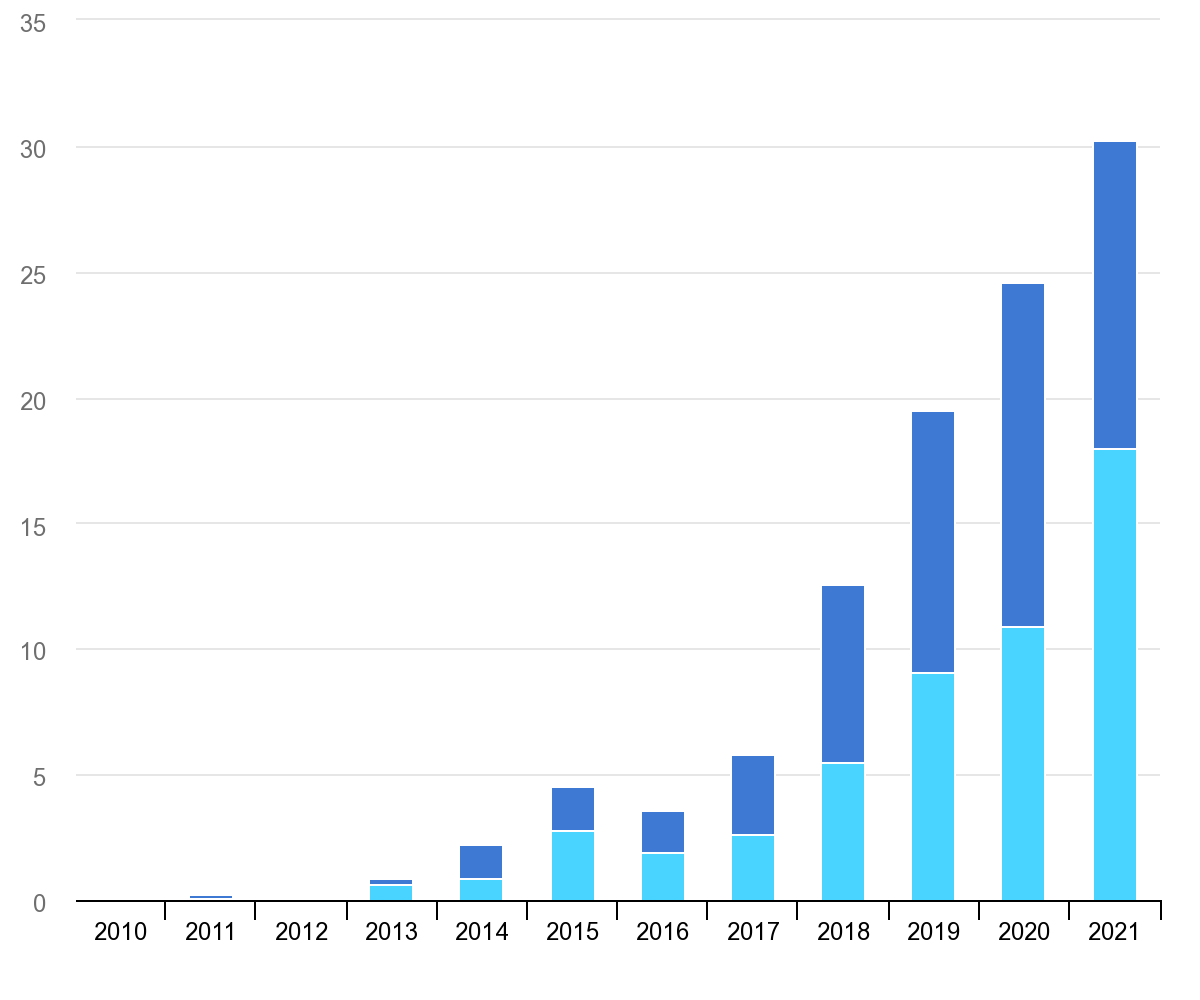
\includegraphics[width=6cm]{images/iea-PPAbysector-2010-2021.png}
      {\scriptsize
      Renewable energy capacity procured with power purchase agreements globally~[GW]. \\
      ICT sector (dark blue), all other sectors (light blue)}
    \end{column}
  
    \source{\href{https://www.iea.org/reports/data-centres-and-data-transmission-networks}{Image: IEA 2022}}
    \end{columns}

  }
\end{frame}


\begin{frame}{Why is this important? 2/2}

  {\footnotesize

  \begin{columns}[T]

    \begin{column}{6cm}
      \centering
      \vspace{.5cm}
      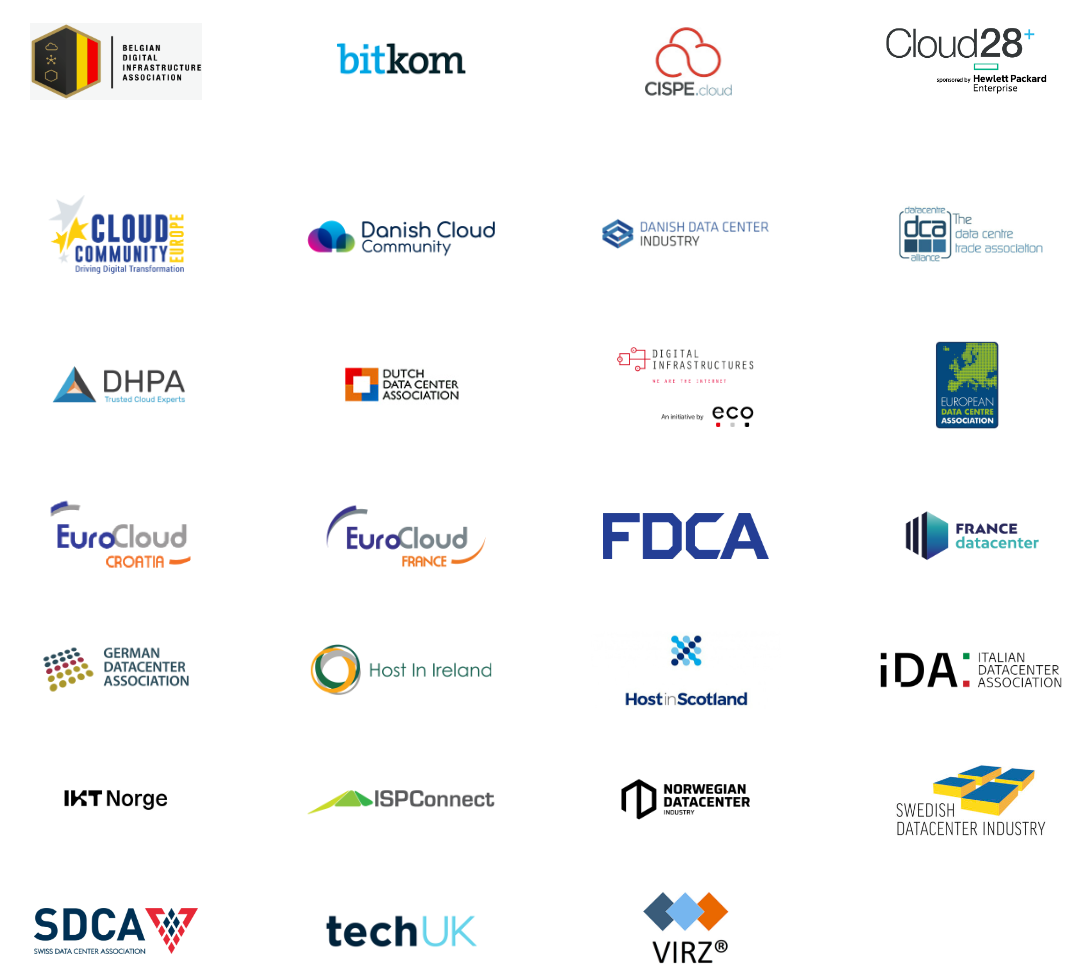
\includegraphics[width=6cm]{images/climateneutraldatacentre.png}
      {\scriptsize
      Data centre operators (Pact Associations) that signed \\ 
      the Climate Neutral Data Centre Pact}
    \end{column}

    \begin{column}{9cm}

      \begin{itemize}
        \item  The initiatives to measure and reduce the environmental impacts of digital infrastructure is spanning far beyond big companies like Google and  Microsoft.
        
        \item In 2021, over 100 data data centre operators and industry associations in Europe signed \hrefc{https://www.climateneutraldatacentre.net/}{the Climate Neutral Data Centre Pact} aiming to make data centres climate neutral by 2030. The pledged targets include measures to increase power usage effectiveness and carbon-free energy supply. The CFE target is declared to be "[..] 75\% of renewable energy or hourly carbon-free energy by December 31, 2025 and 100\% by December 31, 2030." 

        \item Considering (i) a constant growth of a global internet traffic, (ii) a large electricity consumption of data centers distributed in power grids worldwide, and (iii) the need to rapidly decarnonise electricity systems across the globe, it is \alert{important to understand the possible efficiency benefits that space-time load shifting flexibility can provide for the 24/7 carbon-free energy paradigm}. 

      \end{itemize}
      \end{column}
  

    \source{\href{Image: https://www.climateneutraldatacentre.net/signatories/}{Image: climateneutraldatacentre.net/signatories/}}
    \end{columns}

  }
\end{frame}



\begin{frame}{A growing body of research}

  {\footnotesize
  \begin{itemize}

  \item The unique characteristics of data centers as electricity consumers and the active interest of ICT sector companies in sustainable energy drive a growing interest in the research community. Among many other, \hrefc{https://doi.org/10.1016/j.simpat.2015.01.005}{Wang et al. (2015)}, \hrefc{https://doi.org/10.1016/j.comcom.2014.03.004}{Toosi et al. (2017)},
  \hrefc{https://doi.org/10.1016/j.future.2018.03.049}{Grange et al. (2018)},
  \hrefc{https://doi.org/10.1016/j.comcom.2014.03.004}{Velasco et al. (2018)}, and
  \hrefc{https://doi.org/10.1016/j.jcss.2020.11.004}{He \& Shen (2021)} investigated selected aspects of spatial or temporal demand management strategies in the context of supplying data centers power demand with intermittent renewable energy supply. 
  
  \item \hrefc{https://doi.org/10.1016/j.apenergy.2022.119930}{Zhang \& Zavala (2022)} elaborated a mathematical problem that captures both spatial \& temporal load-shifting flexibility provided by data centers. The authors suggest market clearing formulation treats data centers as prosumers that simultaneously request load and provide a load-shifting flexibility service to the grid. The illustrated clearing formulation satisfies fundamental economic properties of the competitive markets, such as revenue adequacy and cost recovery.

  \item The Google research team published a paper on \hrefc{https://doi.org/10.1109/TPWRS.2022.3173250}{Carbon-Aware Computing for Datacenters} \href{https://doi.org/10.1109/TPWRS.2022.3173250}{(Radovanović~et~al.~(2023})). The paper introduced methodology and principles behind a carbon-intelligent compute management system, which minimizes electricity-based carbon footprint and power infrastructure costs by shifting temporally flexible workloads for all datacenter clusters across Google's fleet.

  \end{itemize}
  }

\end{frame}



\begin{frame}{Focus of the study}


  {\footnotesize
  \begin{itemize}
    \item In this study, we explore the potential benefits for 24/7 carbon-free energy buyers and rest of energy system associated with demand flexibility. We aim to answer the following quesitons: \\

    \vspace{0.1cm}
    -- How can demand flexibility reduce the \alert{resources} and \alert{cost-premium} for 24/7~CFE matching?\\ 
    -- How can demand flexibility promote \alert{economic efficiency}?\\
    -- What are the \alert{individual effects} of spatial and temporal demand flexibility, as well what are the synergies from their co-optimiastion? \\
    -- How would advanced technologies, such as long duration storage, affect \alert{the value of demand flexibility}?

    \item For this purpose, we elaborate the mathematical model developed in the previous study, by including spatial and temporal demand flexibility provided by electricity consumers following 24/7~CFE goal. Thus, a flexible 24/7 participant could benefit from \alert{co-optimising} utilisation of available demand flexibility (across space and/or time) and procurement strategies to match every kWh of electiricty consumption with carbon-free energy around-the-clock \alert{more efficiently}.
    
    \item The modelling exercise in this study is focused on \textit{data centers}, i.e., facilities used to house networked computer servers that store, process and distribute large amounts of data. Nevertheless, the findings of this study are likely to be of interest to a wide range of companies and organisations with flexible demand and an interest in 24/7 carbon-free energy procurement, as well as to energy industry experts and stakeholders with an empirical interest in the European energy system.

  \end{itemize}

  }

\end{frame}


%----------------------------------------
%----------------------------------------

\section{Methodology}


\begin{frame}
  \frametitle{A quick overview}

{\footnotesize
  \begin{itemize}
    
    \item The optimization model is based on \hrefc{https://github.com/PyPSA/pypsa-eur}{PyPSA-Eur} -- a widely-used open-source model of the European energy system.

    \item We build upon the mathematical model of 24/7~CFE procurement developed in the former work of authors: \hrefc{https://zenodo.org/record/7180097}{System-level impacts of 24/7 carbon-free electricity procurement in Europe} (October 2022)
    
    \item In this study, we encode a set of new equations and routines, which allow for modelling spatial (computing jobs migration) and temporal (computing jobs scheduling) load flexibility provided by data centers.

    \item We place data centers (i.e., electricity consumers committed to 24/7~CFE goals) in a 
    selection of European countries: Ireland, Denmark, Germany, Finland, and Portugal. These countries have different weather patterns, renewable potentials, national energy and climate policies, legacy fleets of generation capacities, degree of interconnectons, etc. 
    Apart form that, we consider several CFE procurement targets, various degrees of data center flexibility, and two palettes of CFE generation technologies available for 24/7 consumers. These differences help to understand and generalize the interplay of demand flexibility and 24/7~CFE procurement.

  \end{itemize}
}

\end{frame}


\begin{frame}
  \frametitle{PyPSA: an energy modelling ecosystem}

\begin{columns}[T]
\begin{column}{7cm}

{\footnotesize
  \begin{itemize}
  \item \hrefc{https://pypsa.org/}{pypsa.org} project provides a free, user-friendly and performant model environment to support a smooth energy transition around the world. 
  \item The project includes individual packages that enable to go all the way from data processing (e.g., calculating renewable energy potentials or collecting energy assets data) to creating complex energy optimization problems. 
  \item All packages are build in a modular sense so that they may be used independently from each other but interact easily.
  \item PyPSA development and maintenance is coordinated by the Department of Energy Systems @ TU~Berlin \hrefc{https://www.tu.berlin/en/ensys/about-us}{(ENSYS)}.  
  \end{itemize}
}
\end{column}
\begin{column}{9cm}

\centering
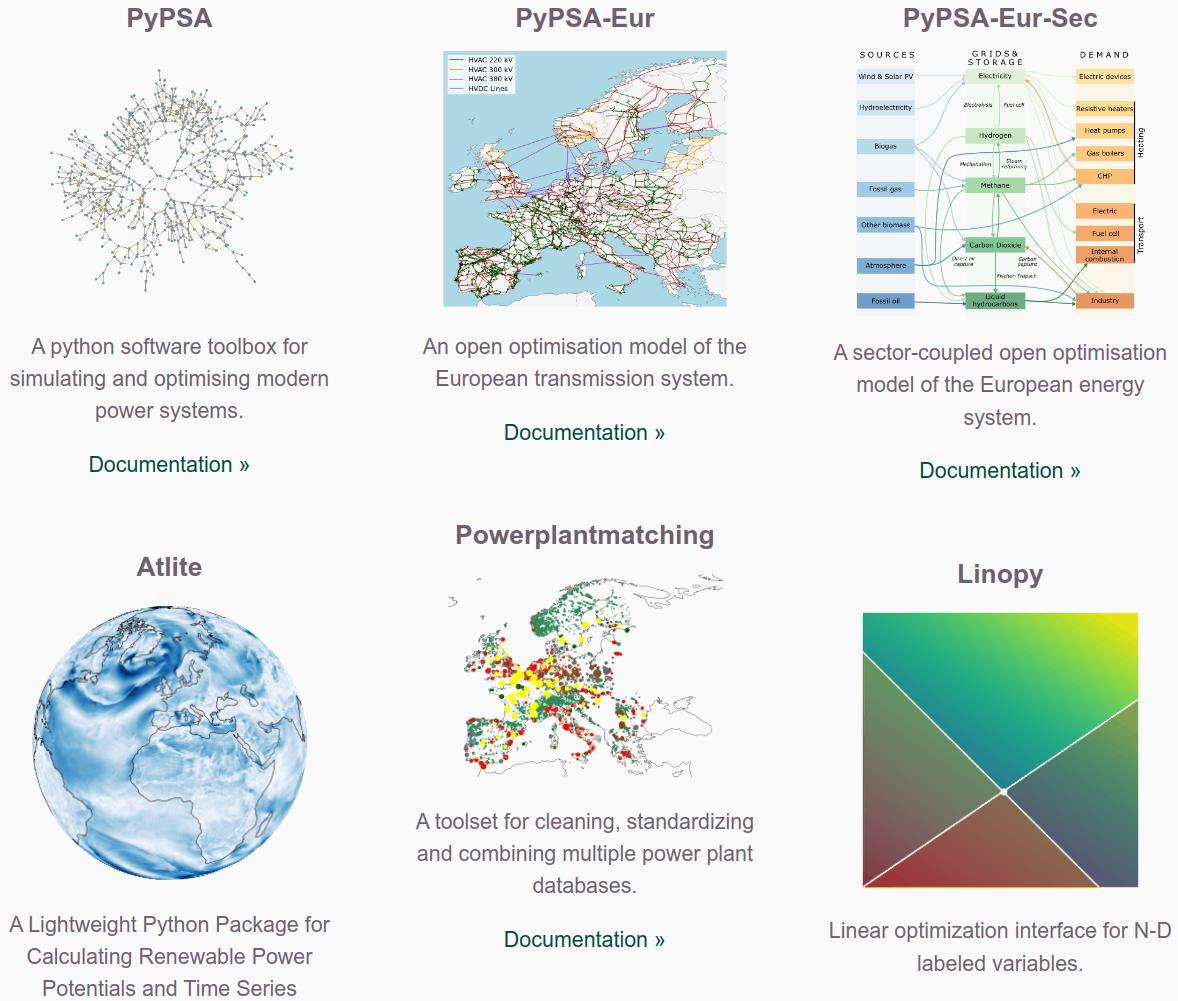
\includegraphics[width=8.5cm]{images/pypsa-web.png}
\source{\href{https://pypsa.org/}{Image: pypsa.org}}

\end{column}
\end{columns}

\end{frame}


% \item PyPSA is used worldwide by dozens of research institutes and companies.\\
% See \hrefc{https://pypsa.readthedocs.io/en/latest/users.html}{list of users}.


\begin{frame}
  \frametitle{Energy system model}

  \begin{columns}[T]
  \begin{column}{7cm}
  {\footnotesize
  \begin{itemize}
  \item This study is done with a modified version of \alert{PyPSA-Eur} -- an open optimisation model of the European energy system.
  \item Automated and configurable software pipeline enables scientific workflow from freely available and open raw input data to optimised electricity system. 
  \item The PyPSA-Eur model is suitable both for operational studies, as well as generation and transmission expansion planning studies. 
  \item  PyPSA-Eur is an open-source project: \\
  \faGithub~\hrefc{https://github.com/PyPSA/pypsa-eur}{PyPSA-Eur on GitHub} \\
  \faBook~\hrefc{https://pypsa-eur.readthedocs.io/en/latest/}{Documentation} \\
  \faLink~\hrefc{https://docs.google.com/presentation/d/1mzj4X9uuO58gUvkhVMRCFWOJUWbs6NR9SNZe-RIkkNo/edit?usp=sharing}{Feature summary} 
  \end{itemize}
  }
  \end{column}

  \begin{column}{9cm}
    \centering
    \vspace{0.1cm}
    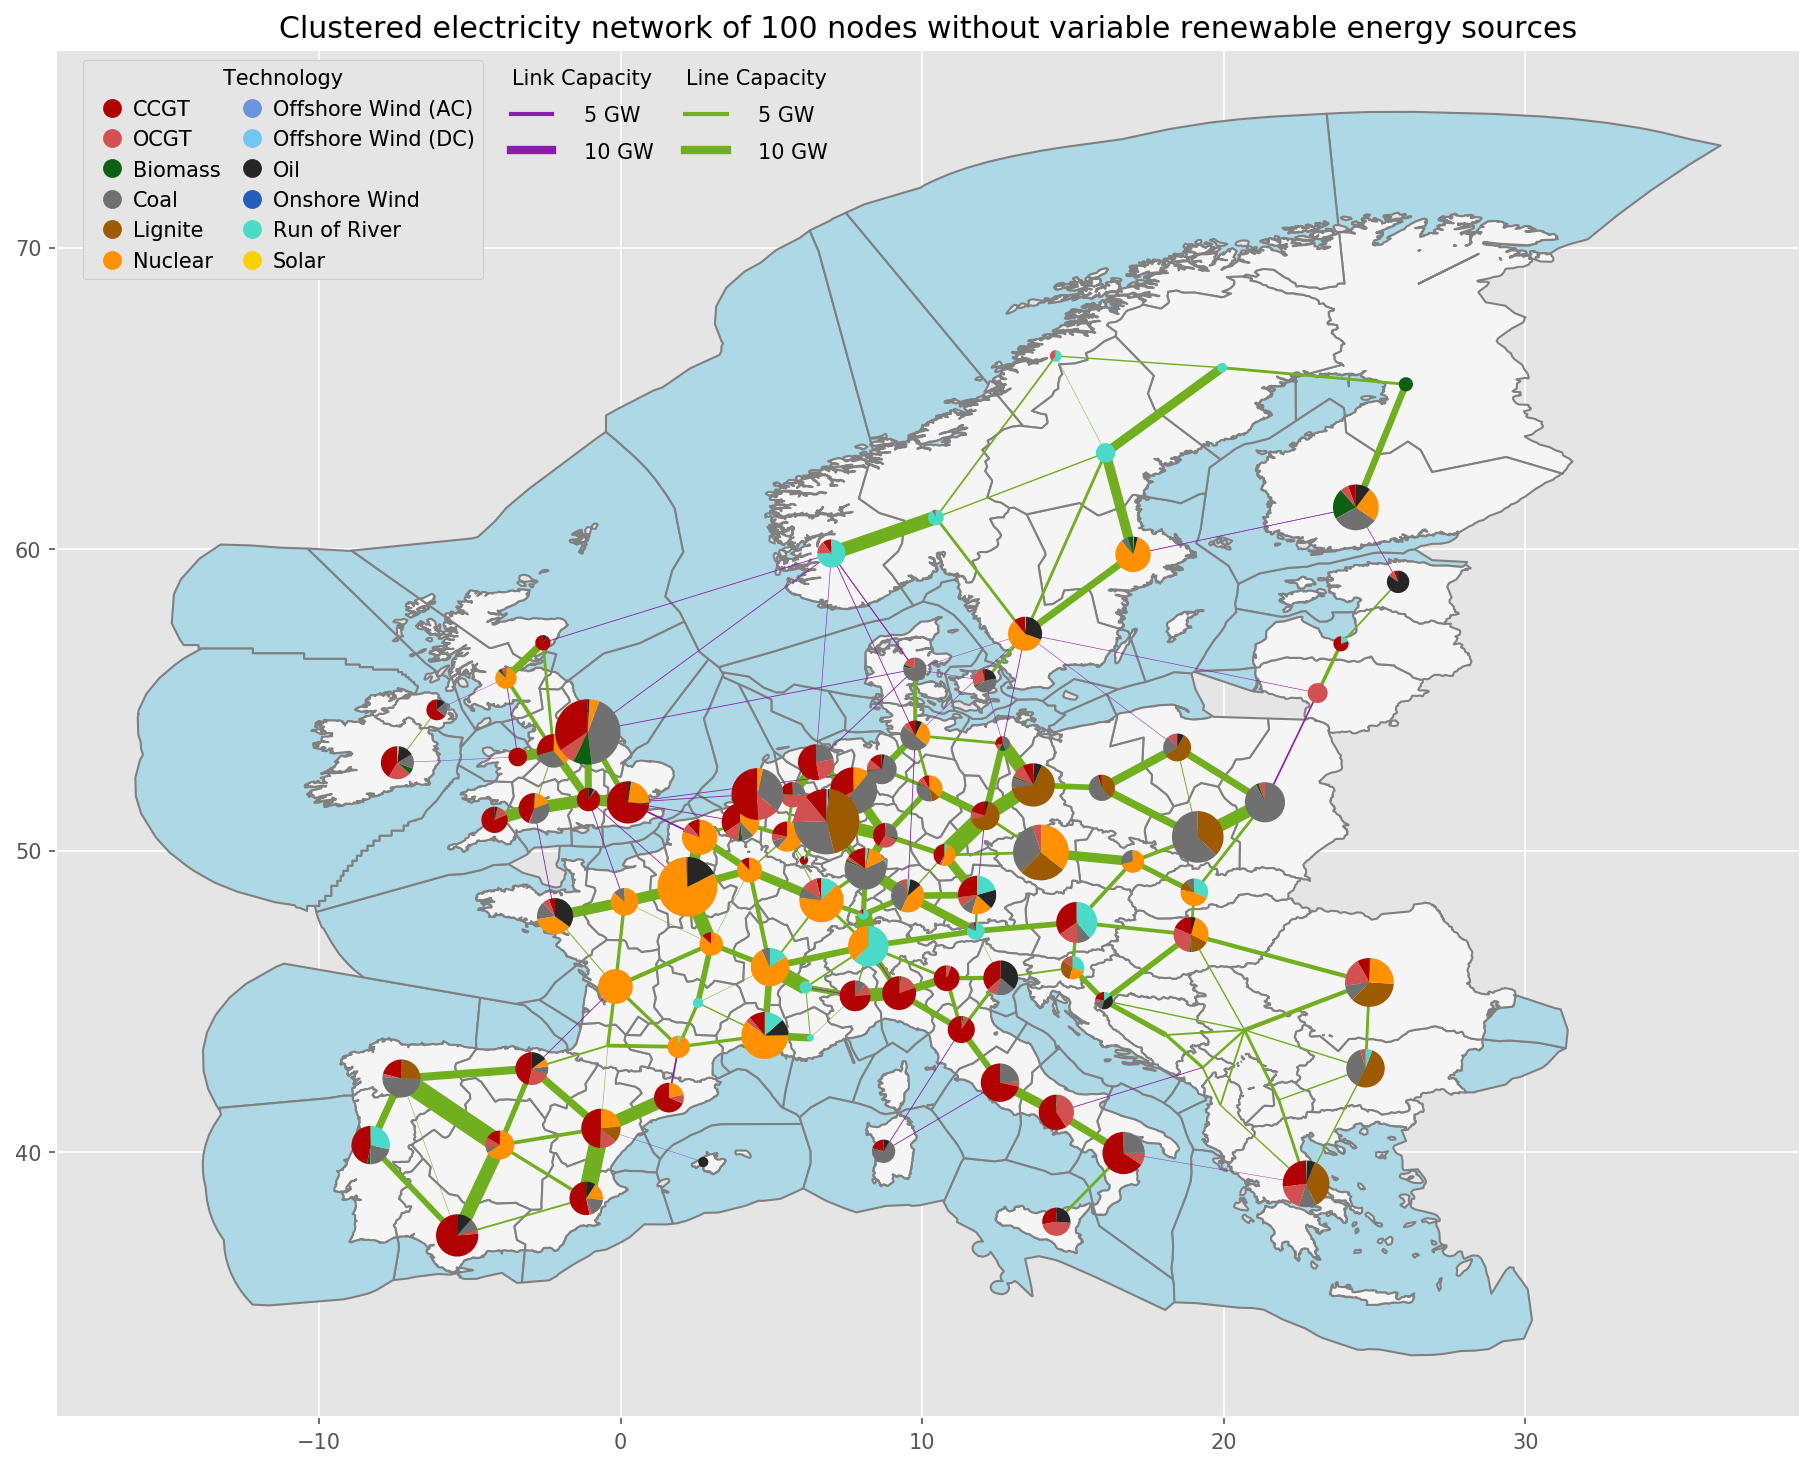
\includegraphics[width=8cm]{images/elec_s_100.png}
  \end{column}
  \end{columns}

  \source{Image: \href{https://github.com/PyPSA/pypsa-eur}{github.com/PyPSA/pypsa-eur}}
\end{frame}



\begin{frame}{Mathematical model of 24/7 CFE procurement}

  {\footnotesize
  \begin{itemize}
  \item The mathematical model of 24/7~CFE procurement is based on the former work of authors: \hrefc{https://zenodo.org/record/7180097}{System-level impacts of 24/7 carbon-free electricity procurement in Europe} published in October 2022. The study included mathematics additional to the PyPSA-Eur model to encode a situation when a fraction of C\&I consumers in a selected European countries commit to the 24/7~CFE goals. The resulting problem optimized investment and operational decisions to meet projected electricity demand for the 24/7~CFE consumers, as well as the demand of other consumers in the European electricity system, while meeting all relevant engineering, reliability, and policy constraints.
  
  \item In this study, we enhance the mathematical model of 24/7~CFE procurement 
  by considering demand flexibility that can take form of \alert{temporal} (computing jobs scheduling) and \alert{spatial} (computing jobs migration) load shifting by data centers. 
  
  \item Thus, a data center operator (i.e., a flexible consumer following 24/7~CFE goal) can meet a given CFE target by either procuring energy generation and storage assets directly, and buying electricity from a local grid in hours when electricity mix is sufficiently clean  (like in the previous study), as well as utilize spatial and/or temporal flexibility to achieve hourly matching of demand with clean electricity more efficiently.

  \end{itemize}
  }

\end{frame}



\begin{frame}{Matching electricity supply and demand: a case of inflexible consumer}

  {\footnotesize
  The model optimizes a portfolio of carbon-free generation and storage technologies 
  procured by the C\&I consumers that commit to 24/7~CFE goal. The portfolio assets have to be located in the same market zone.

  The hourly demand of 24/7 participating consumer $d_t$ for hour $t$ can be met by a combination of the following: \\
    \begin{itemize}
      \item dispatch $g_{r,t}$ of procured carbon-free generators $r\in CFE$ 
      \item dispatch $\bar{g}_{s,t}$ of procured storage technologies $s\in STO$
            (requires charge $\ubar{g}_{s,t}$)
      \item imports of electricity from the grid $im_t$.
    \end{itemize}

  \begin{columns}
  \begin{column}{8cm}
  \begin{equation}
  \sum_{r\in CFE} g_{r,t} + \sum_{s\in STO} \left(\bar{g}_{s,t} - \ubar{g}_{s,t}\right) - ex_t + im_t  =  d_t \hspace{.7cm} \forall t
  \label{eqn:inflexnb}
  \end{equation}

  \vspace{0.3cm}
  NB: the excess from the local supply $ex_t$ can either be sold to the grid at market prices or curtailed.
  \end{column}

\begin{column}{5cm}
\centering
{\small
\begin{circuitikz}
  \draw (0,13.5) to [short,i^=$im_t$]  (1.5,13.5) to (1.5,13);
  \draw [ultra thick] (0,13) node[anchor=south]{} -- (4,13);
  \draw(2.5,13) |- +(0,0.5) to [short,i^=$ex_t$] +(1.5,0.5);
  \draw (0.5,13) -- +(0,-0.5) node[sground]{};
  \draw (2,12) node[vsourcesinshape, rotate=270](V2){}
  (V2.left) -- +(0,0.6);
  \draw (3.5,13) -- (3.5,12.4);
  \draw (3.5,12.4) to [esource] (3.5,11.7);
  \draw (0.5,11.3) node{$d_t$};
  \draw (2,11.3) node{$g_{CFE,t}$};
  \draw (3.5,11.3) node{$g_{STO,t}$};
\end{circuitikz}
}
\end{column}
\end{columns}

}
\end{frame}



\begin{frame}{24/7 CFE matching: a case of inflexible consumer}

  {\footnotesize

  The \alert{24/7 CFE matching} is modelled with a constraint (\ref{eqn:CFE}), 
  which matches demand of participating consumers with carbon-free resources on an hourly basis.  The constraint ensures that sum over generators from procured CFE resources $r\in CFE$, discharge and charge from storage technologies $s\in STO$,
  as well as import from the grid $im_t$ multiplied by the grid's CFE factor $CFE_t$
  must be higher or equal than a certain \alert{CFE score} $x$ multiplied with the total load $d_t$:
  \vspace{0.1cm}
  \begin{equation}
  \sum_{r\in CFE, t\in T} g_{r,t} + \sum_{s\in STO, t\in T} \left(\bar{g}_{s,t} - \ubar{g}_{s,t}\right) - \sum_{t\in T} ex_t + \sum_{t\in T} CFE_t \cdot im_t \geq x \cdot \sum_{t\in T} d_t
  \label{eqn:CFE}
  \end{equation}

  \vspace{0.3cm}

  \begin{columns}[T]
    \begin{column}{7.5cm}
    \centering  
    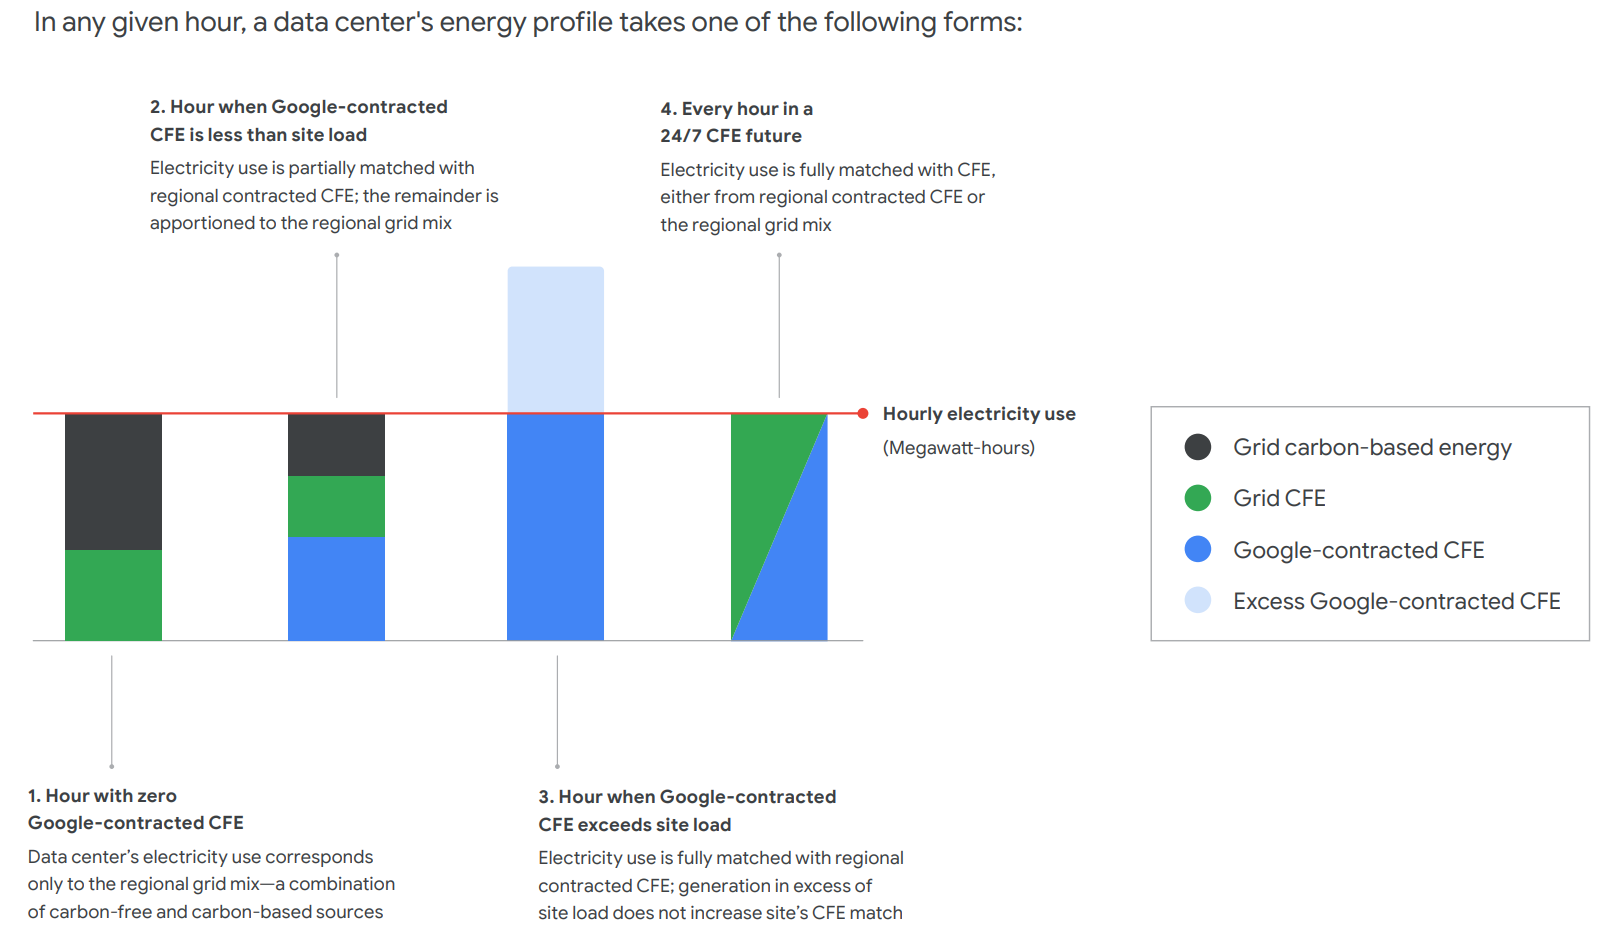
\includegraphics[width=8cm]{images/247-concept.png}
    \end{column}
    \begin{column}{6cm}
    \vspace{0.3cm}
      \noindent\fbox{%
      \parbox{\textwidth}{%
    The \alert{CFE score} $x$~[\%] measures the degree to which hourly electricity consumption is matched with carbon-free electricity generation within the regional grid.
    The matric is calculated using both CFE contracted by 24/7 participant, as well as CFE coming from the regional grid mix. \\
    \\
    The 24/7 CFE matching concept is aligned with \hrefc{https://www.gstatic.com/gumdrop/sustainability/24x7-carbon-free-energy-methodologies-metrics.pdf}{24/7 CFE: Methodologies and Metrics} paper by Google.
    }} 

    \end{column}
    \end{columns}
    }
\source{Image: \href{https://www.gstatic.com/gumdrop/sustainability/24x7-carbon-free-energy-methodologies-metrics.pdf}{24/7 CFE: Methodologies and Metrics}, Google 2021}    
\end{frame}


\begin{frame}{24/7 CFE matching: grid CFE factor}

  {\footnotesize

  The \alert{grid CFE factor} $CFE_t$ in eq. (\ref{eqn:CFE}) defines the percentage of clean electricity in each MWh of imported electricity from the grid to supply participating 24/7 loads in a given hour. The factor depends on the generation mix in the region where 24/7 participant is located, as well as on the generation mix in other regions from which electricity is imported to the local region ($import_t$).

  \begin{columns}
    \begin{column}{8cm}
    Using notation on the right, the average cleanness of the rest of the electricity system is:   
  \begin{equation*}
  ImportCFE_t = \frac{A_t}{A_t + D_t}
  \end{equation*}

  The CFE factor of grid supply\footnote{\scriptsize{Generators contracted by 24/7 consumers (C) are excluded from the grid supply.}} for a given hour $t$ is:

  \begin{equation*}
  CFE_t = \frac{B_t + ImportCFE_t * import_t}{B_t + E_t + import_t}
  \end{equation*}    

  \end{column}
  \begin{column}{5cm}
  \centering
  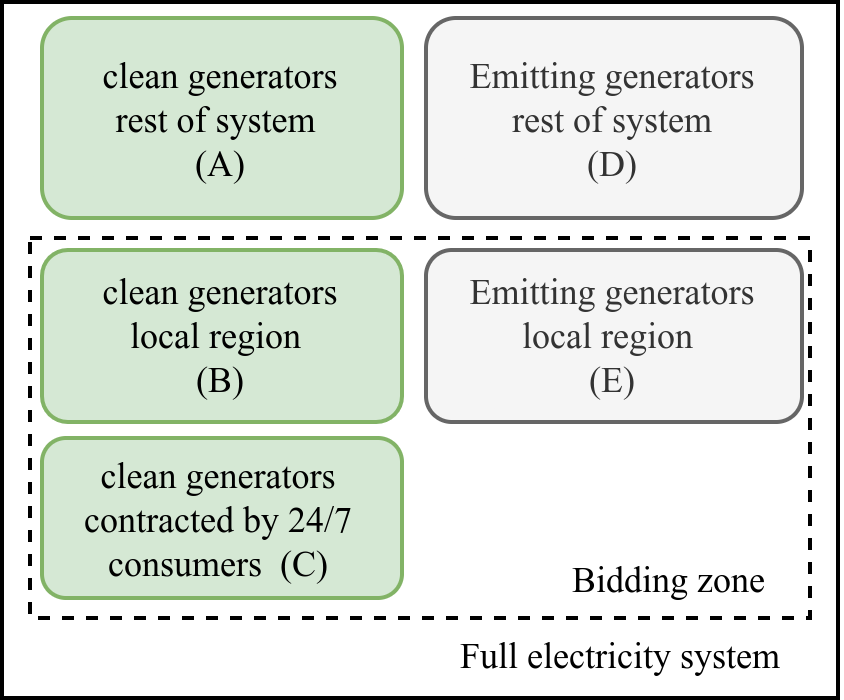
\includegraphics[width=4.5cm]{images/cfe.png} \\
  \scriptsize{Here we follow \hrefc{https://acee.princeton.edu/24-7/}{Xu et al. (2021)}}
  \end{column}
    
  \end{columns}
  \noindent\fbox{%
  \parbox{\textwidth}{%
  \scriptsize{
  Note that the grid CFE factor is affected by capacity procured by 24/7 consumers. This
  introduces a nonconvex term to the optimization problem. The nonconvexity can be avoided by treating the grid CFE factor as a parameter that is iteratively updated (starting with $CFE_t =0 \,~\forall t$). In the previous study, we concluded that one forward pass (i.e. 2 iterations) yields very good convergence. This observation holds true also for the optimization problem behind this study with multiple 24/7 consumers.}
  }}
  }
  
\end{frame}



\begin{frame}{24/7 CFE matching: excess CFE}

  {\footnotesize

  The \alert{excess CFE} represents generation from the procured resources above consumption of the 24/7 participant in a particular hour.  The excess CFE \alert{is not counted toward the CFE score} -- and thus it is subtracted on the left-hand side of the eq. (\ref{eqn:CFE}). While it does not contribute to the CFE Score, excess CFE could potentially be stored (using batteries) and shifted to another hour, sold to the regional grid at {\bf market prices}, or curtailed. 

  \vspace{0.2cm}

  The total amount of CFE exported to the regional grid is constrained to a certain level on an annual basis. The export limit ($ExLimit$) is set to 20\% of annual 24/7 participating consumer's demand. 
  Thus, constraint (\ref{eqn:excess}) gives the 24/7 participant flexibility to sell electricity to the regional grid, while avoiding the situation that sales to the grid become significantly larger than CFE supply to own demand.
  
  \begin{equation}
  \sum_{t\in T} export_t \leq ExLimit \cdot \sum_{t\in T} d_t
  \label{eqn:excess}
  \end{equation}

  \vspace{0.2cm}
  \noindent\fbox{%
  \parbox{\textwidth}{%
  The {\bf market prices} are derived from the dual variable of each zone's
  \hrefc{https://pypsa.readthedocs.io/en/latest/components.html}{energy balance constraint}. An infinitely small relaxation of the constraint, i.e., one unit of load less to be met, returns the marginal costs of providing that unit, which can be used as the electricity price indicator in a competitive market.
  }}
  }

\end{frame}



\begin{frame}{Implementation of data center load flexibility}

{\footnotesize
  \begin{columns}[T]

  \begin{column}{6cm}
  \centering
  \vspace{0.2cm}
  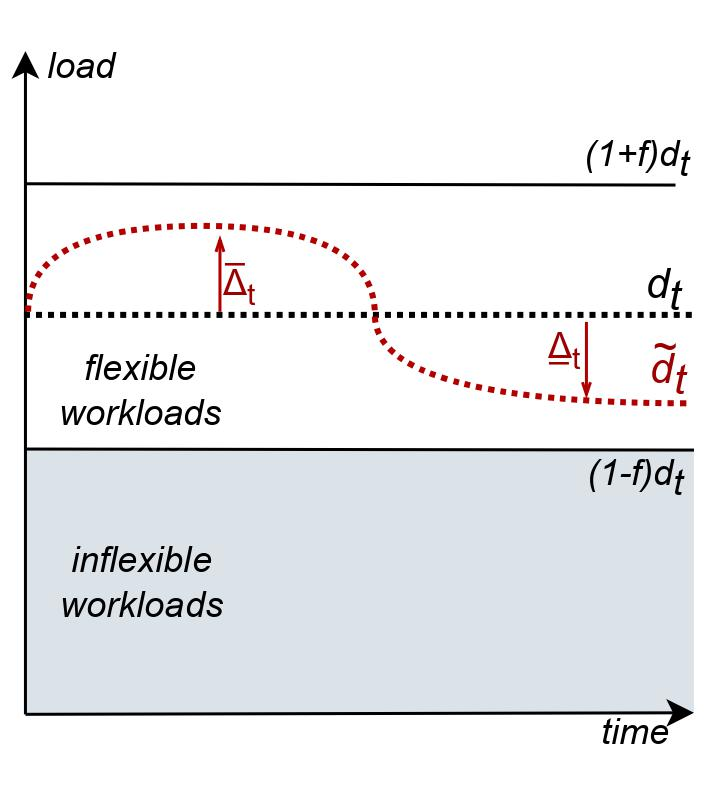
\includegraphics[width=6cm]{images/drawio_flexrange_d.pdf}
  \end{column}

  \begin{column}{9cm}
  \begin{itemize}

  \item The premise of data center flexibility is that a known amount of computing jobs, and assosiated power usage is "flexible", i.e., electricity loads can potentially be shifted in space (across datacenter locations), or to other times (by delaying jobs' execution).\footnote{{\scriptsize A change in cluster-level CPU usage can be accurately mapped into a change in its power usage, see \href{https://arxiv.org/abs/2106.11750}{Radovanovic et al. (2021)}}}

  \item Thus, the \alert{requested load $\widetilde{d}_t$} of a data center can deviate from the nominal load $d_t$. The requested load $\widetilde{d}_t$ is constrained by the data center capacity (an upper limit) and the inflexible loads (a lower limit).
  
  \item The range of possible deviations of the requested and nominal loads is assumed to lie within $f$~[\%] of the nominal load, such as:\\
  \begin{equation*}
  [1-f] \cdot d_t \le  d_t + (\overline{\Delta}_t - \underline{\Delta}_t) \le [1+f] \cdot d_t \quad \forall t \in T
  \label{eqn:range}
  \end{equation*}
  
  \vspace{0.1cm}
  \noindent where $\overline{\Delta}_t, \underline{\Delta}_t \in \mathbb{R}_{+}$ stand for positive/negative deviation of $\widetilde{d}_t$ and $d_t$ in hour $t$.
  \end{itemize}

  \end{column}
  \end{columns}
}
\end{frame}



%%%%%%%%%%%%%%%%%%%%%%%%%%%%%%%%%%%%%%%%%%%%%%%%%%%%%%%%%%%%%%%%%%%%%%%
\begin{frame}{Spatial load shifting problem 1/3}

  {\footnotesize

  We introduce a concept of \alert{spatial load management system} that allows for shifting workloads across locations. The load shifts take place via \alert{virtual links} -- non-physical pathways between data center nodes (\href{https://doi.org/10.1016/j.apenergy.2022.119930}{Zhang \& Zavala (2022)}).

  \centering
  \hspace*{0.7cm}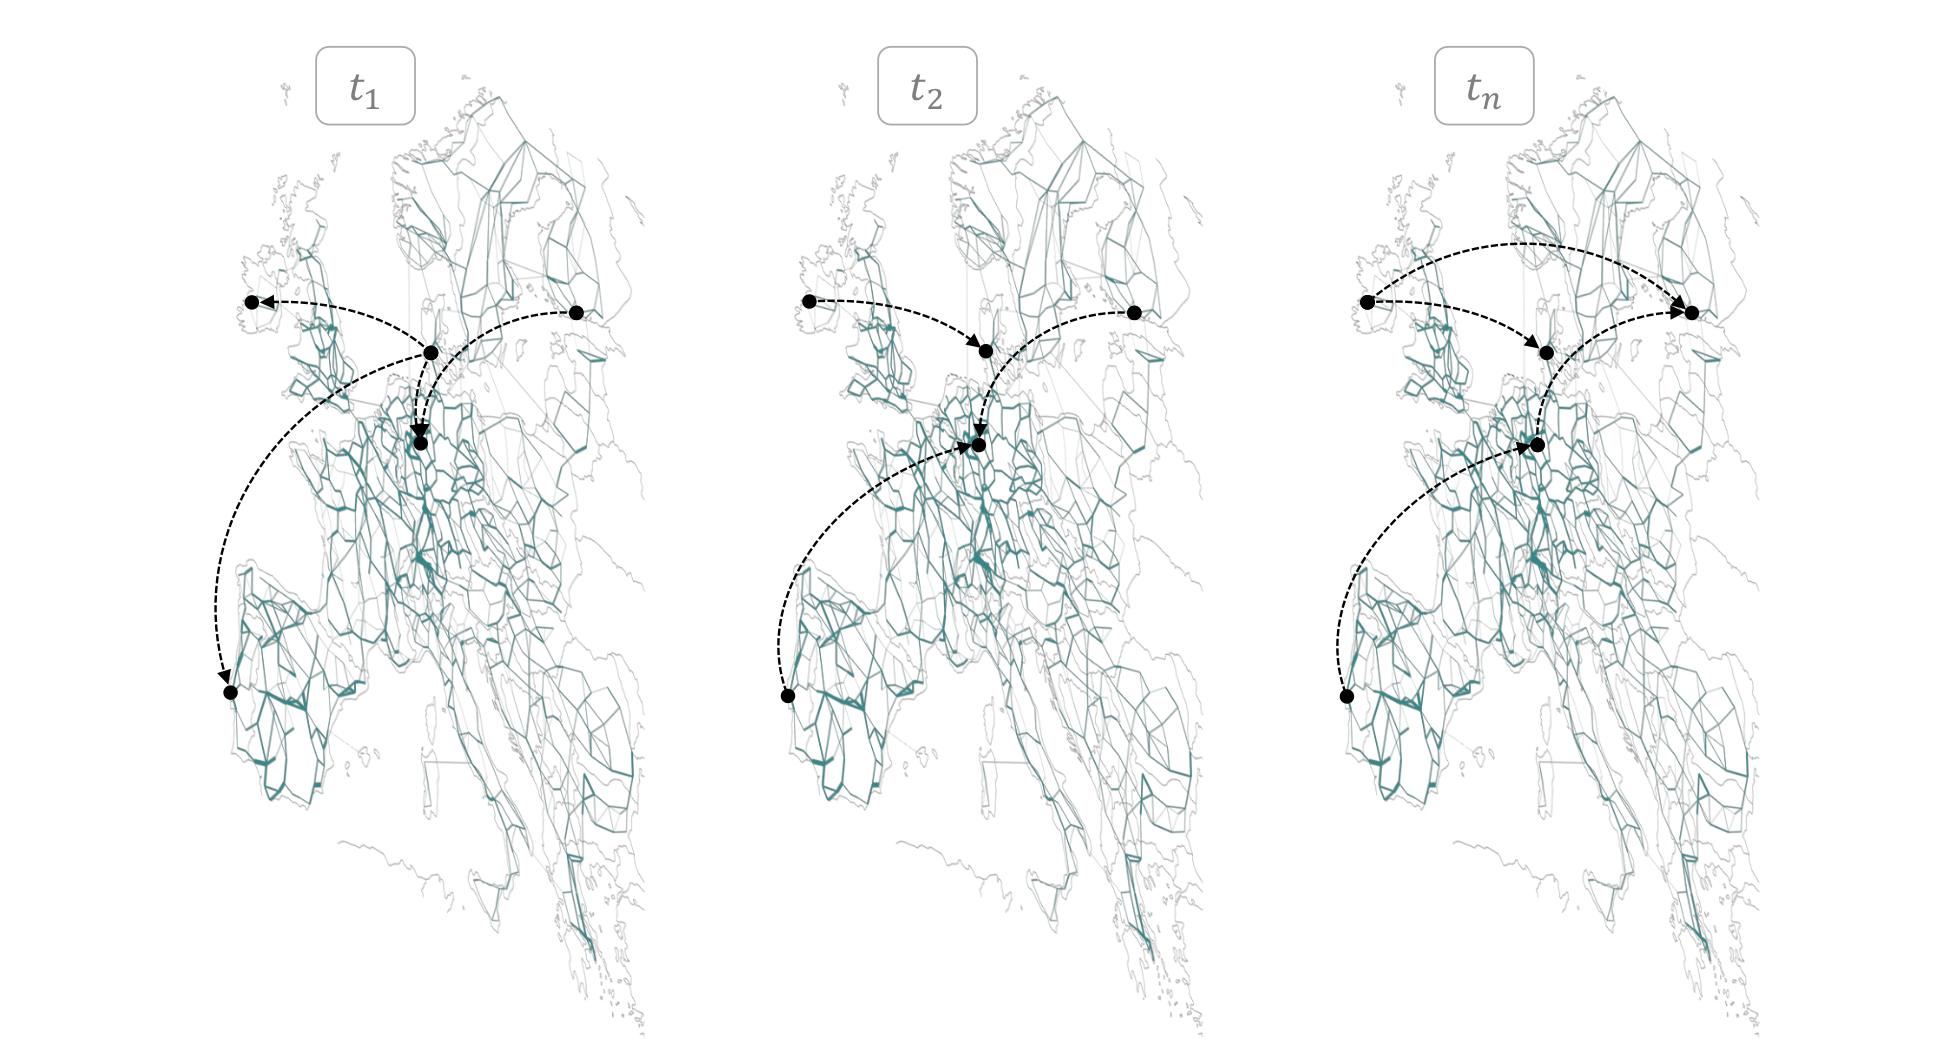
\includegraphics[width=12cm]{images/spatial-vlinks.png}
  }
\end{frame}


\begin{frame}{Spatial load shifting problem 2/3}

  {\footnotesize

  We introduce a concept of \alert{spatial load management system} that allows for shifting workloads across locations. The load shifts take place via \alert{virtual links} -- non-physical pathways between data center nodes (\href{https://doi.org/10.1016/j.apenergy.2022.119930}{Zhang \& Zavala (2022)}).

  Let $\Theta$ be the set of all virtual links; let $\delta_\vartheta \in \mathbb{R}_{+}$ be load shifts (flows via virtual pathways); and let $N_{DC}$ be the set of data centers (flexible consumers). We can define $\Theta_n^{snd} := \{\vartheta \in \Theta | snd(\vartheta) = n\} \subseteq \Theta$, $\Theta_n^{rec} := \{\vartheta \in \Theta | rec(\vartheta) = n\} \subseteq \Theta$ to be the set of sending and receiving virtual links at node $n \in N_{DC}$. 

  The nodal energy balance defined for inflexible consumers (eq.~\ref{eqn:inflexnb}) is now extended by variables representing shifts of load \alert{across locations}, since the requested load at a given node can include shifts to/from other data center nodes: 

  \begin{columns}
    \begin{column}{8cm}
      \begin{equation}
        \begin{split}
     & \sum_{r\in CFE} g_{r,n,t} + \sum_{s\in STO} \left(\bar{g}_{s,n,t} - \ubar{g}_{s,n,t}\right) - ex_{n,t} + im_{n,t}  = \\
     & \textcolor{TUred}{d_{n,t} + \sum_{\vartheta \in \Theta_n^{rec}}\delta_{\vartheta, t} - \sum_{\vartheta \in \Theta_n^{snd}}\delta_{\vartheta, t}} \hspace{.5cm} \forall n \in N_{DC}, t \in T 
        \end{split}
      \label{eqn:spatialnb}
      \end{equation}
    \end{column}
  \begin{column}{5cm}
  \centering
  {\small
  \begin{circuitikz}
    \draw (0,13.5) to [short,i^=$im_{n,t}$]  (1.5,13.5) to (1.5,13);
    \draw [ultra thick] (0,13) node[anchor=south]{} -- (4,13);
    \draw(2.5,13) |- +(0,0.5) to [short,i^=$ex_{n,t}$] +(1.5,0.5);
    \draw (0.5,13) -- +(0,-0.5) node[sground]{};
    \draw (2,12) node[vsourcesinshape, rotate=270](V2){}
    (V2.left) -- +(0,0.6);
    \draw (3.5,13) -- (3.5,12.4);
    \draw (3.5,12.4) to [esource] (3.5,11.7);
    \draw (0.5,11.3) node{\textcolor{TUred}{$\widetilde{d_{n,t}}$}};
    \draw (2,11.3) node{$g_{CFE,n,t}$};
    \draw (3.5,11.3) node{$g_{STO,n,t}$};
  \end{circuitikz}
  }
  \end{column}
  \end{columns}
  }
\end{frame}


\begin{frame}{Spatial load shifting problem 3/3}

  {\footnotesize
  \begin{columns}

    \begin{column}{6cm}
      Computing capacity constraints (eq. \ref{eqn:spatialflex}) ensure that the requested load at each data center  $\widetilde{d}_{n,t}$ does not exceed available capacity (an upper limit, eq. \ref{eqn:spatialb}), as well as that a certain data center does not shift load that exceeds flexible jobs share (a lower limit, eq. \ref{eqn:spatialc}).
    \end{column}

  \begin{column}{7cm}
    \begin{subequations}
      \begin{align}
          \widetilde{d_{n,t}} &=  d_{n,t} + \sum_{\vartheta \in \Theta_n^{rec}}\delta_{\vartheta, t} - \sum_{\vartheta \in \Theta_n^{snd}}\delta_{\vartheta, t} \quad \forall n \in N_{DC}, t \in T \label{eqn:spatiala} \\
          \widetilde{d_{n,t}} &\le [1+f] \cdot d_{n,t}  \quad \forall n \in N_{DC}, t \in T \label{eqn:spatialb} \\
          \widetilde{d_{n,t}} &\ge [1-f] \cdot d_{n,t}  \quad \forall n \in N_{DC}, t \in T \label{eqn:spatialc}
      \end{align}
      \label{eqn:spatialflex}
      \end{subequations}
  \end{column}
  \end{columns}

  \vspace{-0.1cm}
  NB spatial load shifts are not subject to any eletricity network transmission constraints; as such, the only source of congestion for the virtual links is computing capacity constraints (i.e., availability of flexible workloads). \\

  \vspace{0.1cm}
  The 24/7~CFE matching constraint for inflexible consumer (eq. \ref{eqn:CFE}) is now defined over a set of data center nodes $n \in N_{DC}$ and is extended on the right-hand side by spatial load shifts. Thus, flexible consumer can benefit from an additional degree of freedom that helps relaxing the constraint for locations and times when providing demand with carbon-free electricity is difficult:
  \vspace{0.1cm}
  \begin{equation}
    \begin{split}
  &\sum_{r\in CFE, t\in T} g_{r,n,t} + \sum_{s\in STO, t\in T} \left(\bar{g}_{s,n,t} - \ubar{g}_{s,n,t}\right) - \sum_{t\in T} ex_{n,t} + \sum_{t\in T} CFE_{n,t} \cdot im_{n,t} \geq \\ 
  &x_n \cdot \textcolor{TUred}{\sum_{t\in T} \left( d_{n,t} + \sum_{\vartheta \in \Theta_n^{rec}}\delta_{\vartheta, t} - \sum_{\vartheta \in \Theta_n^{snd}}\delta_{\vartheta, t}\right)} \quad \forall n \in N_{DC} \label{eqn:spatialCFE}
    \end{split}
  \end{equation}
  }
  
\end{frame}


%%%%%%%%%%%%%%%%%%%%%%%%%%%%%%%%%%%%%%%%%%%%%%%%%%%%%%%%%%%%%%%%%%%%%%%
\begin{frame}{Temporal load shifting problem 1/3}

  {\footnotesize

  To capture temporal flexibility, we introduce a concept a data center \alert{temporal load management system} that allows for shifting load from a given time to another time point in the future.

  \centering
  \hspace*{0.7cm}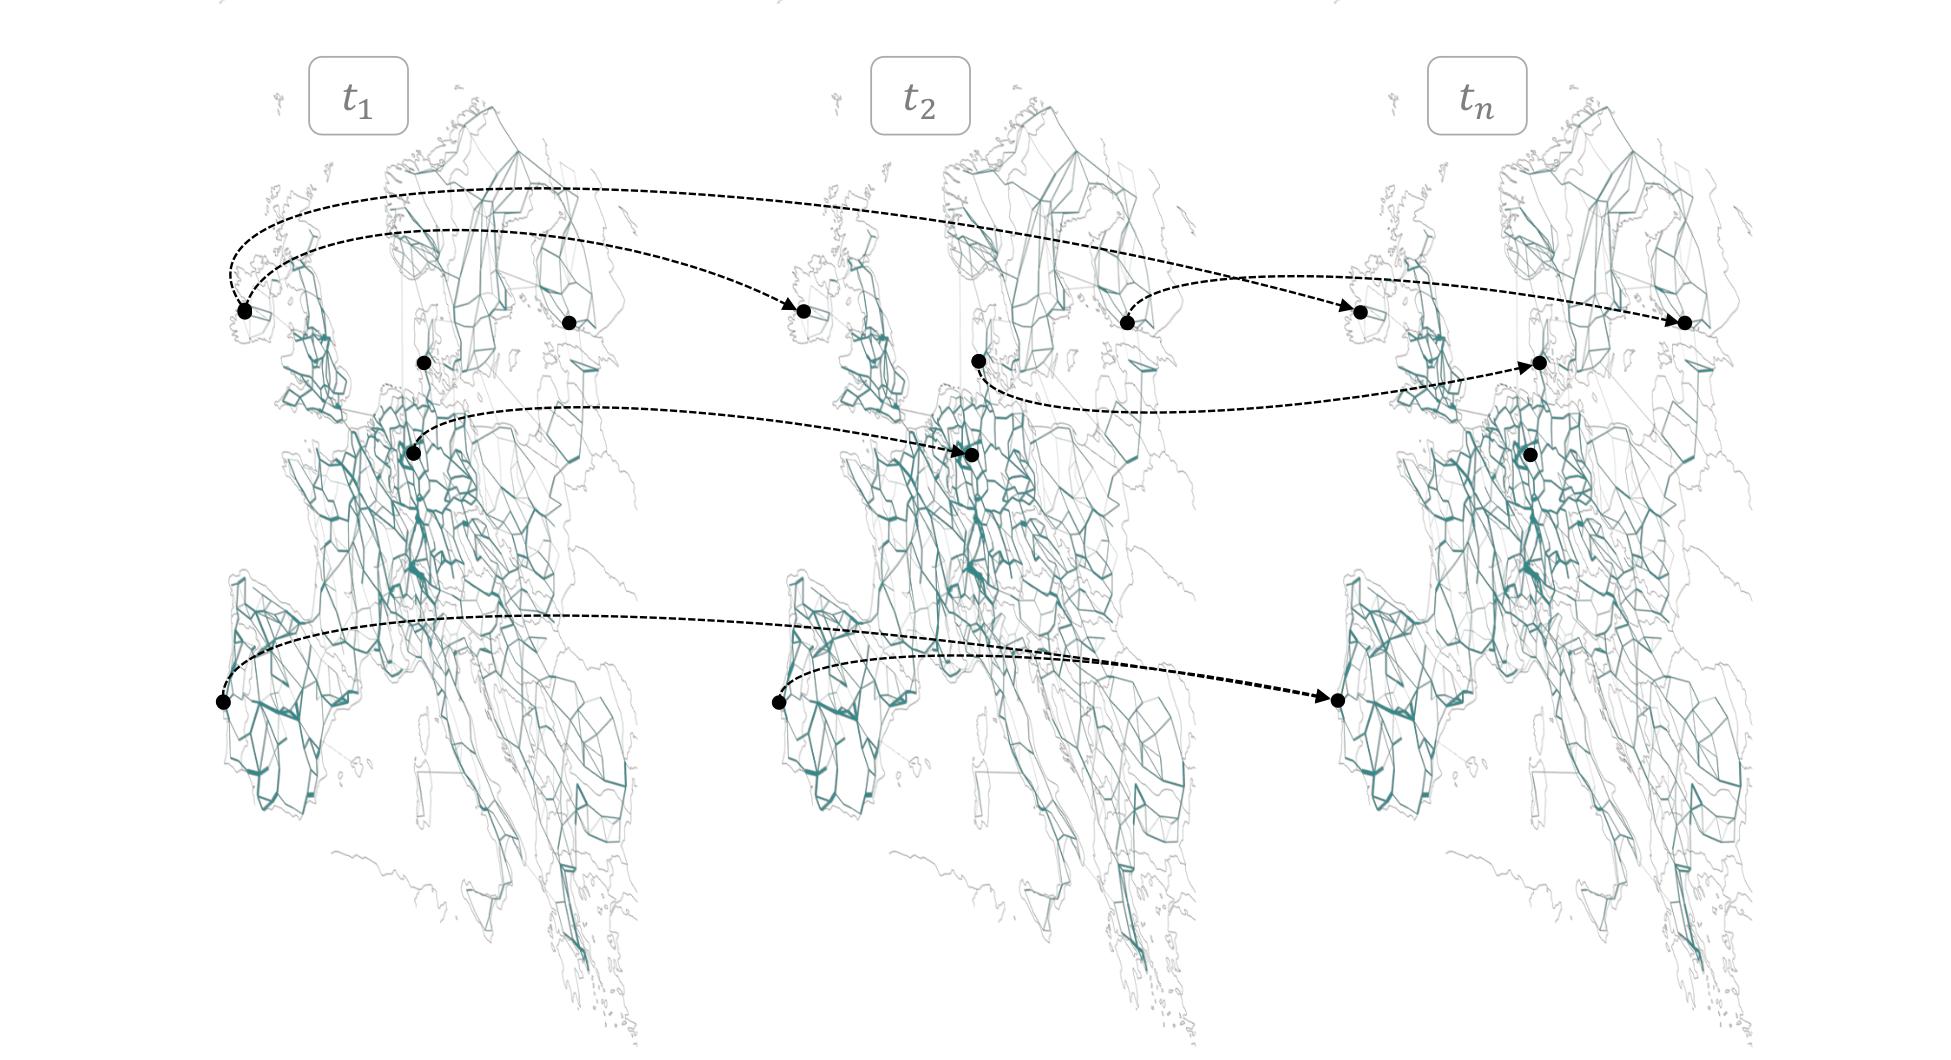
\includegraphics[width=12cm]{images/temporal-vlinks.png}
  }
\end{frame}


\begin{frame}{Temporal load shifting problem 2/2}

  {\footnotesize

  To capture temporal flexibility, we introduce a concept a data center \alert{temporal load management system} that allows for shifting load from a given time to another time point in the future.

  Consider a time horizon of our optimization problem $T = \{t_1 , t_2 , ..., t_T\}$. For simplicity, let us assume that there is a single flexible consumer (i.e., no spatial load shifts) with a demand-side temporal load management mechanism denoted with a singleton set $\{s'\}$. Let variables $\bar{g}_{s',t},\ubar{g}_{s',t} \in \mathbb{R}_{+}$ to be workloads that are resheduled in time, i.e., shifted from a time $t$ to a later time $t'$. Thus, the requested load  $\widetilde{d_{t}}$ of flexible consumer can deviate from the nominal value $d_{n,t}$ due to temporal load management. 
  
  The nodal energy balance is now extended with variables representing shifts of load \alert{across time}:

  \begin{columns}
    \begin{column}{8cm}
      \begin{equation}
        \begin{split}
        &\sum_{r\in CFE} g_{r,t} + \sum_{s\in STO} \left(\bar{g}_{s,t} - \ubar{g}_{s,t}\right) - ex_{t} + im_{t}  = \\
        &\textcolor{TUred}{d_{t} + \sum_{{s'}} \left(\bar{g}_{s',t} - \ubar{g}_{s',t}\right)}\hspace{.5cm} \{N_{DC}\}, \forall t \in T 
        \label{eqn:temporalnb}
        \end{split}
      \end{equation}
      \end{column}
  \begin{column}{5cm}
  \centering
  {\small
  \begin{circuitikz}
    \draw (0,13.5) to [short,i^=$im_{t}$]  (1.5,13.5) to (1.5,13);
    \draw [ultra thick] (0,13) node[anchor=south]{} -- (4,13);
    \draw(2.5,13) |- +(0,0.5) to [short,i^=$ex_{t}$] +(1.5,0.5);
    \draw (0.5,13) -- +(0,-0.5) node[sground]{};
    \draw (2,12) node[vsourcesinshape, rotate=270](V2){}
    (V2.left) -- +(0,0.6);
    \draw (3.5,13) -- (3.5,12.4);
    \draw (3.5,12.4) to [esource] (3.5,11.7);
    \draw (0.5,11.3) node{\textcolor{TUred}{$\widetilde{d_{t}}$}};
    \draw (2,11.3) node{$g_{CFE,t}$};
    \draw (3.5,11.3) node{$g_{STO,t}$};
  \end{circuitikz}
  }
  \end{column}
  \end{columns}
  }
\end{frame}


\begin{frame}{Temporal load shifting problem 3/3}

  {\footnotesize
  \begin{columns}

    \begin{column}{7.2cm}
      Computing capacity constraints for temporal load shifting problem (eq. \ref{eqn:temporalflex}) ensure that workloads delayed to a given time $t$ do not exceed available cluster capacity (an upper limit, eq. \ref{eqn:temporalb}), as well as that only flexible workloads can be shifted in time (a lower limit, eq. \ref{eqn:temporalc}).
    \end{column}

  \begin{column}{5.8cm}
  \begin{subequations}
    \begin{align}
        \widetilde{d_{t}} =  d_{t} + \sum_{{s'}} \left(\bar{g}_{s',t} - \ubar{g}_{s',t}\right)\quad &\forall t \in T  \label{eqn:temporala} \\
        \widetilde{d_{t}} \le [1+f] \cdot d_{t}  \quad &\forall t \in T  \label{eqn:temporalb} \\
        \widetilde{d_{t}} \ge [1-f] \cdot d_{t}  \quad &\forall t \in T  \label{eqn:temporalc}
    \end{align}
    \label{eqn:temporalflex}
    \end{subequations}
  \end{column}
  \end{columns}

  \vspace{-0.1cm}
  We follow \href{https://arxiv.org/abs/2106.11750}{Radovanovic et al. (2021)} implementing the daily usage conservation rule -- an additional constraint to ensure that the cluster-level daily compute usage is preserved when flexible workload is shifted in time:

  \begin{equation}
    \sum_{t | t \in t(DAYS)} \left(\bar{g}_{s',t} - \ubar{g}_{s',t}\right) = 0 \quad \{s'\}
    \label{eqn:dailyconserv}
  \end{equation}

  The 24/7~CFE matching constraint is also extended to account for the temporal load management mechanism. Consumer with temporally flexible loads can benefit from an additional degree of freedom that helps relaxing the 24/7~CFE constraint for the times when providing demand with carbon-free electricity is difficult:
  \vspace{0.1cm}
  \begin{equation}
    \begin{split}
  &\sum_{r\in CFE, t\in T} g_{r,t} + \sum_{s\in STO, t\in T} \left(\bar{g}_{s,t} - \ubar{g}_{s,t}\right) - \sum_{t\in T} ex_{t} + \sum_{t\in T} CFE_{t} \cdot im_{t} \geq \\ 
  &x \cdot \textcolor{TUred}{\sum_{t\in T} \left( d_{t} + \sum_{{s'}}\left(\bar{g}_{s',t} - \ubar{g}_{s',t}\right)\right)} \hspace{.5cm} \{N_{DC}\} 
  \label{eqn:temporalCFE}
    \end{split}
  \end{equation}
  
  }
\end{frame}


%%%%%%%%%%%%%%%%%%%%%%%%%%%%%%%%%%%%%%%%%%%%%%%%%%%%%%%%%%%%%%%%%%%%%%%
\begin{frame}{Spatially-temporal load shifting problem 1/3}
  \centering
  \vspace{0.3cm}
  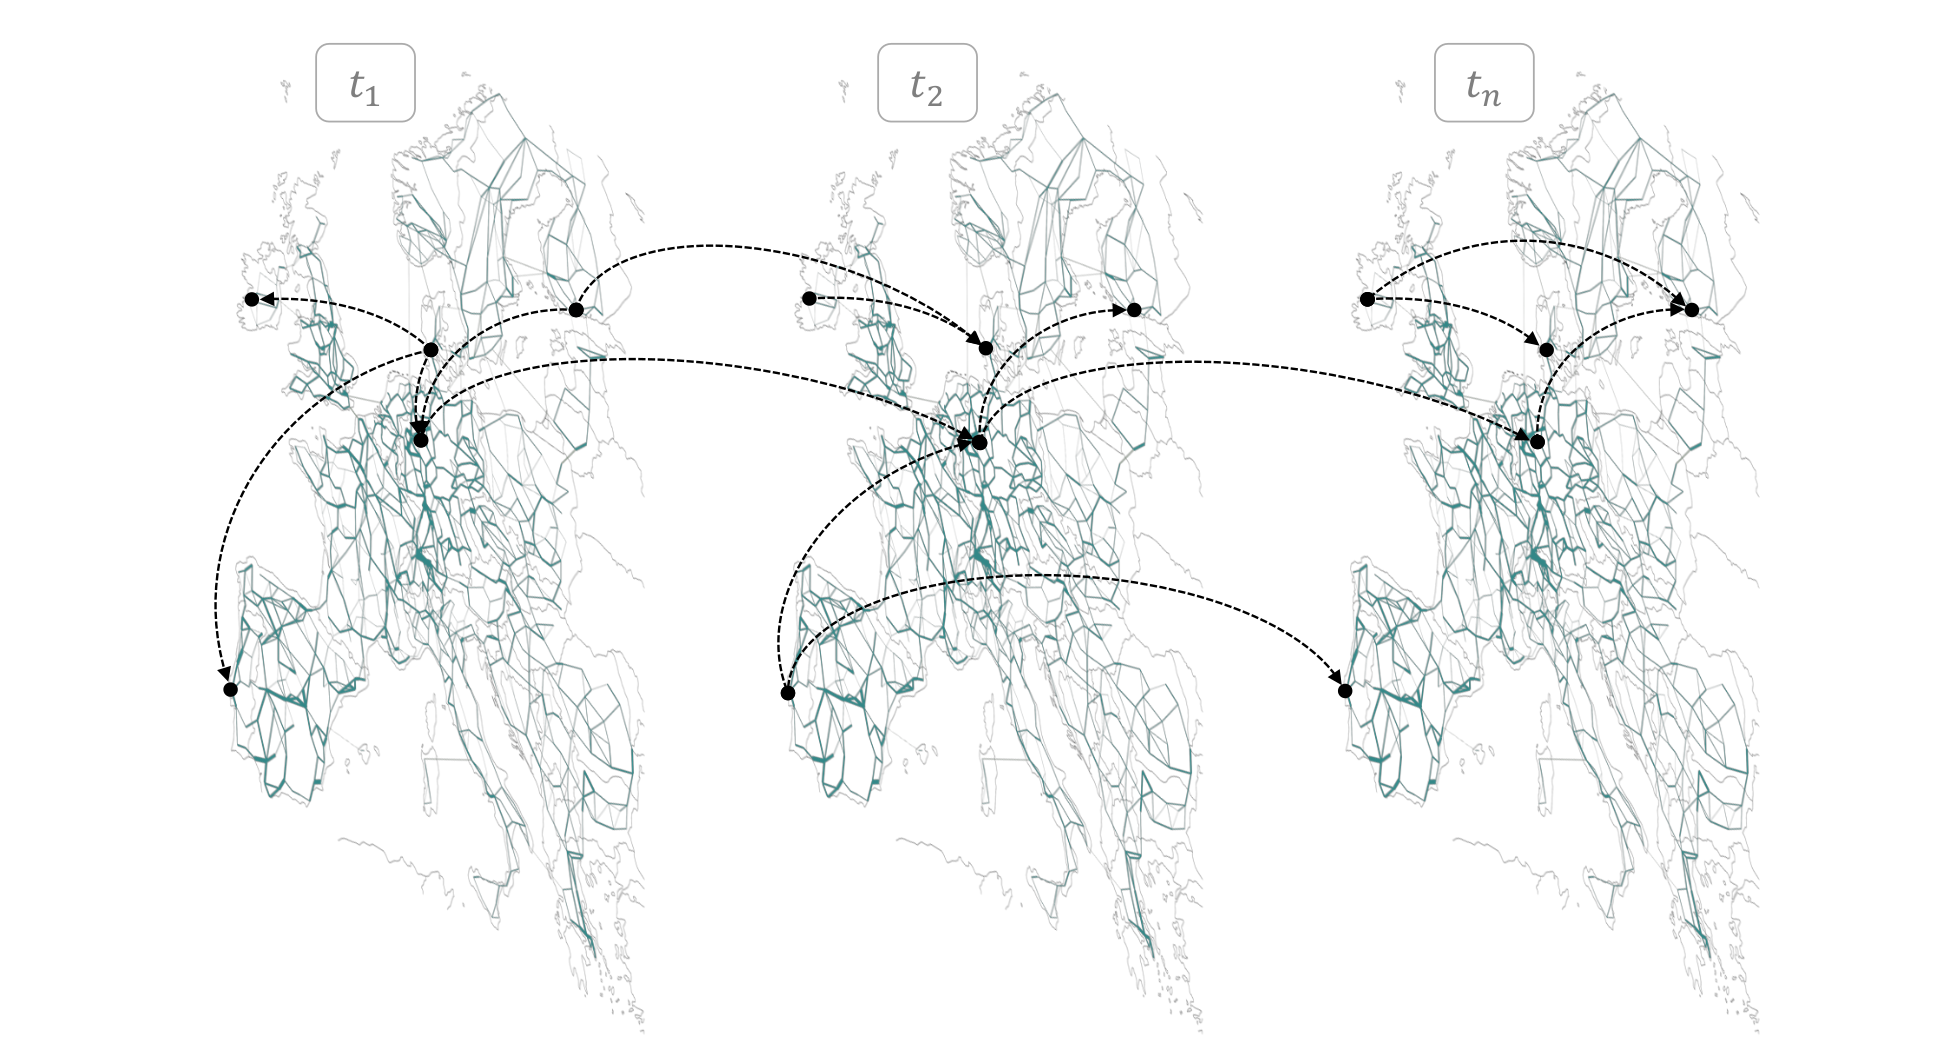
\includegraphics[width=12cm]{images/spatial-temporal-vlinks.png}
\end{frame}


\begin{frame}{Spatially-temporal load shifting problem 2/3}

  {\footnotesize

  The temporal and spatial flexibility of electricity demand can be \alert{co-optimized} to help achieving clean electricity targets. The resulting mathematical problem brings together the formulations of spatial and temporal load management systems shown above.

  We consider a set data centers (flexible consumers) $n \in N_{DC}$ located in various locations within the electricity network. Data centers are interconnected with virtual links $\Theta_n^{snd}, \Theta_n^{rec}$ (complete graph). Each data center also has a temporal load management mechanism $S_n^{dsm} := \{s' \in S | dsm(s') = n\}$.

  The nodal energy balance is adjusted to account for variables represeting load shifts \alert{across space and time}:

  \vspace{0.2cm}
  \begin{columns}
    \begin{column}{9cm}
      \begin{equation}
        \begin{split}
        &\sum_{r\in CFE} g_{r,n,t} + \sum_{s\in STO} \left(\bar{g}_{s,n,t} - \ubar{g}_{s,n,t}\right) - ex_{n,t} + im_{n,t}  = \\
        & \textcolor{TUred}{d_{n,t} + \sum_{\vartheta \in \Theta_n^{rec}}\delta_{\vartheta, t} - \sum_{\vartheta \in \Theta_n^{snd}}\delta_{\vartheta, t} + \sum_{{s'} \in S_n^{dsm}} \left(\bar{g}_{s',n,t} - \ubar{g}_{s',n,t}\right)} \\ 
        & \hspace{.5cm} \forall n \in N_{DC}, t \in T 
        \label{eqn:bothnb}
        \end{split}
      \end{equation}
    \end{column}
  \begin{column}{5cm}
  \centering
  {\small
  \begin{circuitikz}
    \draw (0,13.5) to [short,i^=$im_{n,t}$]  (1.5,13.5) to (1.5,13);
    \draw [ultra thick] (0,13) node[anchor=south]{} -- (4,13);
    \draw(2.5,13) |- +(0,0.5) to [short,i^=$ex_{n,t}$] +(1.5,0.5);
    \draw (0.5,13) -- +(0,-0.5) node[sground]{};
    \draw (2,12) node[vsourcesinshape, rotate=270](V2){}
    (V2.left) -- +(0,0.6);
    \draw (3.5,13) -- (3.5,12.4);
    \draw (3.5,12.4) to [esource] (3.5,11.7);
    \draw (0.5,11.3) node{\textcolor{TUred}{$\widetilde{d_{n,t}}$}};
    \draw (2,11.3) node{$g_{CFE,n,t}$};
    \draw (3.5,11.3) node{$g_{STO,n,t}$};

  \end{circuitikz}
  }
  \end{column}
  \end{columns}
  }
\end{frame}



\begin{frame}{Spatially-temporal load shifting problem 3/3}

  {\footnotesize
  \begin{columns}

    \begin{column}{5cm}
      Computing capacity constraints (eq.~\ref{eqn:bothflex}) now ensure that the requested load at each data center  $\widetilde{d}_{n,t}$ does not exceed the limits for each data center $n \in N_{DC}$ considering both spatial and temporal load shifts at each time point $t$.
    \end{column}

  \begin{column}{8cm}
    \begin{subequations}
      \begin{align}
        \begin{split}
          &\widetilde{d_{n,t}} =  d_{n,t} + \sum_{\vartheta \in \Theta_n^{rec}}\delta_{\vartheta, t} - \sum_{\vartheta \in \Theta_n^{snd}}\delta_{\vartheta, t} \\
          &+ \sum_{{s'} \in S_n^{dsm}} \left(\bar{g}_{s',n,t} - \ubar{g}_{s',n,t}\right) \quad \forall n \in N_{DC}, t \in T \\
        \end{split}
        \label{eqn:botha} \\
        &\widetilde{d_{n,t}} \le [1+f] \cdot d_{n,t}  \quad \forall n \in N_{DC}, t \in T \label{eqn:bothb} \\
        &\widetilde{d_{n,t}} \ge [1-f] \cdot d_{n,t}  \quad \forall n \in N_{DC}, t \in T \label{eqn:bothc}
      \end{align}
      \label{eqn:bothflex}
      \end{subequations}
  \end{column}
  \end{columns}

  Daily compute usage conservation rule is applied to each data center:
  \begin{equation}
    \sum_{t | t \in t(DAYS)} \left(\bar{g}_{s',t} - \ubar{g}_{s',t}\right) = 0 \quad \forall {s'} \in S_n^{dsm}
    \label{eqn:dailyconserv2}
  \end{equation}

  Finally, the 24/7~CFE matching constraint is adjusted accordingly. With co-optimization of temporal or spatial load shifting, flexibility can be harnessed to achieve clean electricity targets more efficiently:
  \vspace{0.1cm}
  \begin{equation}
    \begin{split}
  &\sum_{r\in CFE, t\in T} g_{r,n,t} + \sum_{s\in STO, t\in T} \left(\bar{g}_{s,n,t} - \ubar{g}_{s,n,t}\right) - \sum_{t\in T} ex_{n,t} + \sum_{t\in T} CFE_{n,t} \cdot im_{n,t} \geq \\ 
  &x_n \cdot \textcolor{TUred}{\sum_{t\in T} \left( d_{n,t} + \sum_{\vartheta \in \Theta_n^{rec}}\delta_{\vartheta, t} - \sum_{\vartheta \in \Theta_n^{snd}}\delta_{\vartheta, t} + \sum_{{s'} \in S_n^{dsm}} \left(\bar{g}_{s',n,t} - \ubar{g}_{s',n,t}\right)\right)}\quad \forall n \in N_{DC} \label{eqn:spatialCFE}
    \end{split}
  \end{equation}
  }
  
\end{frame}


%----------------------------------------
%----------------------------------------
\section{Study design}


\begin{frame}{Study design: European power system}
  
  {\footnotesize
  \begin{columns}[T]

  \begin{column}{7cm}
  \centering
  \vspace{0.5cm}
  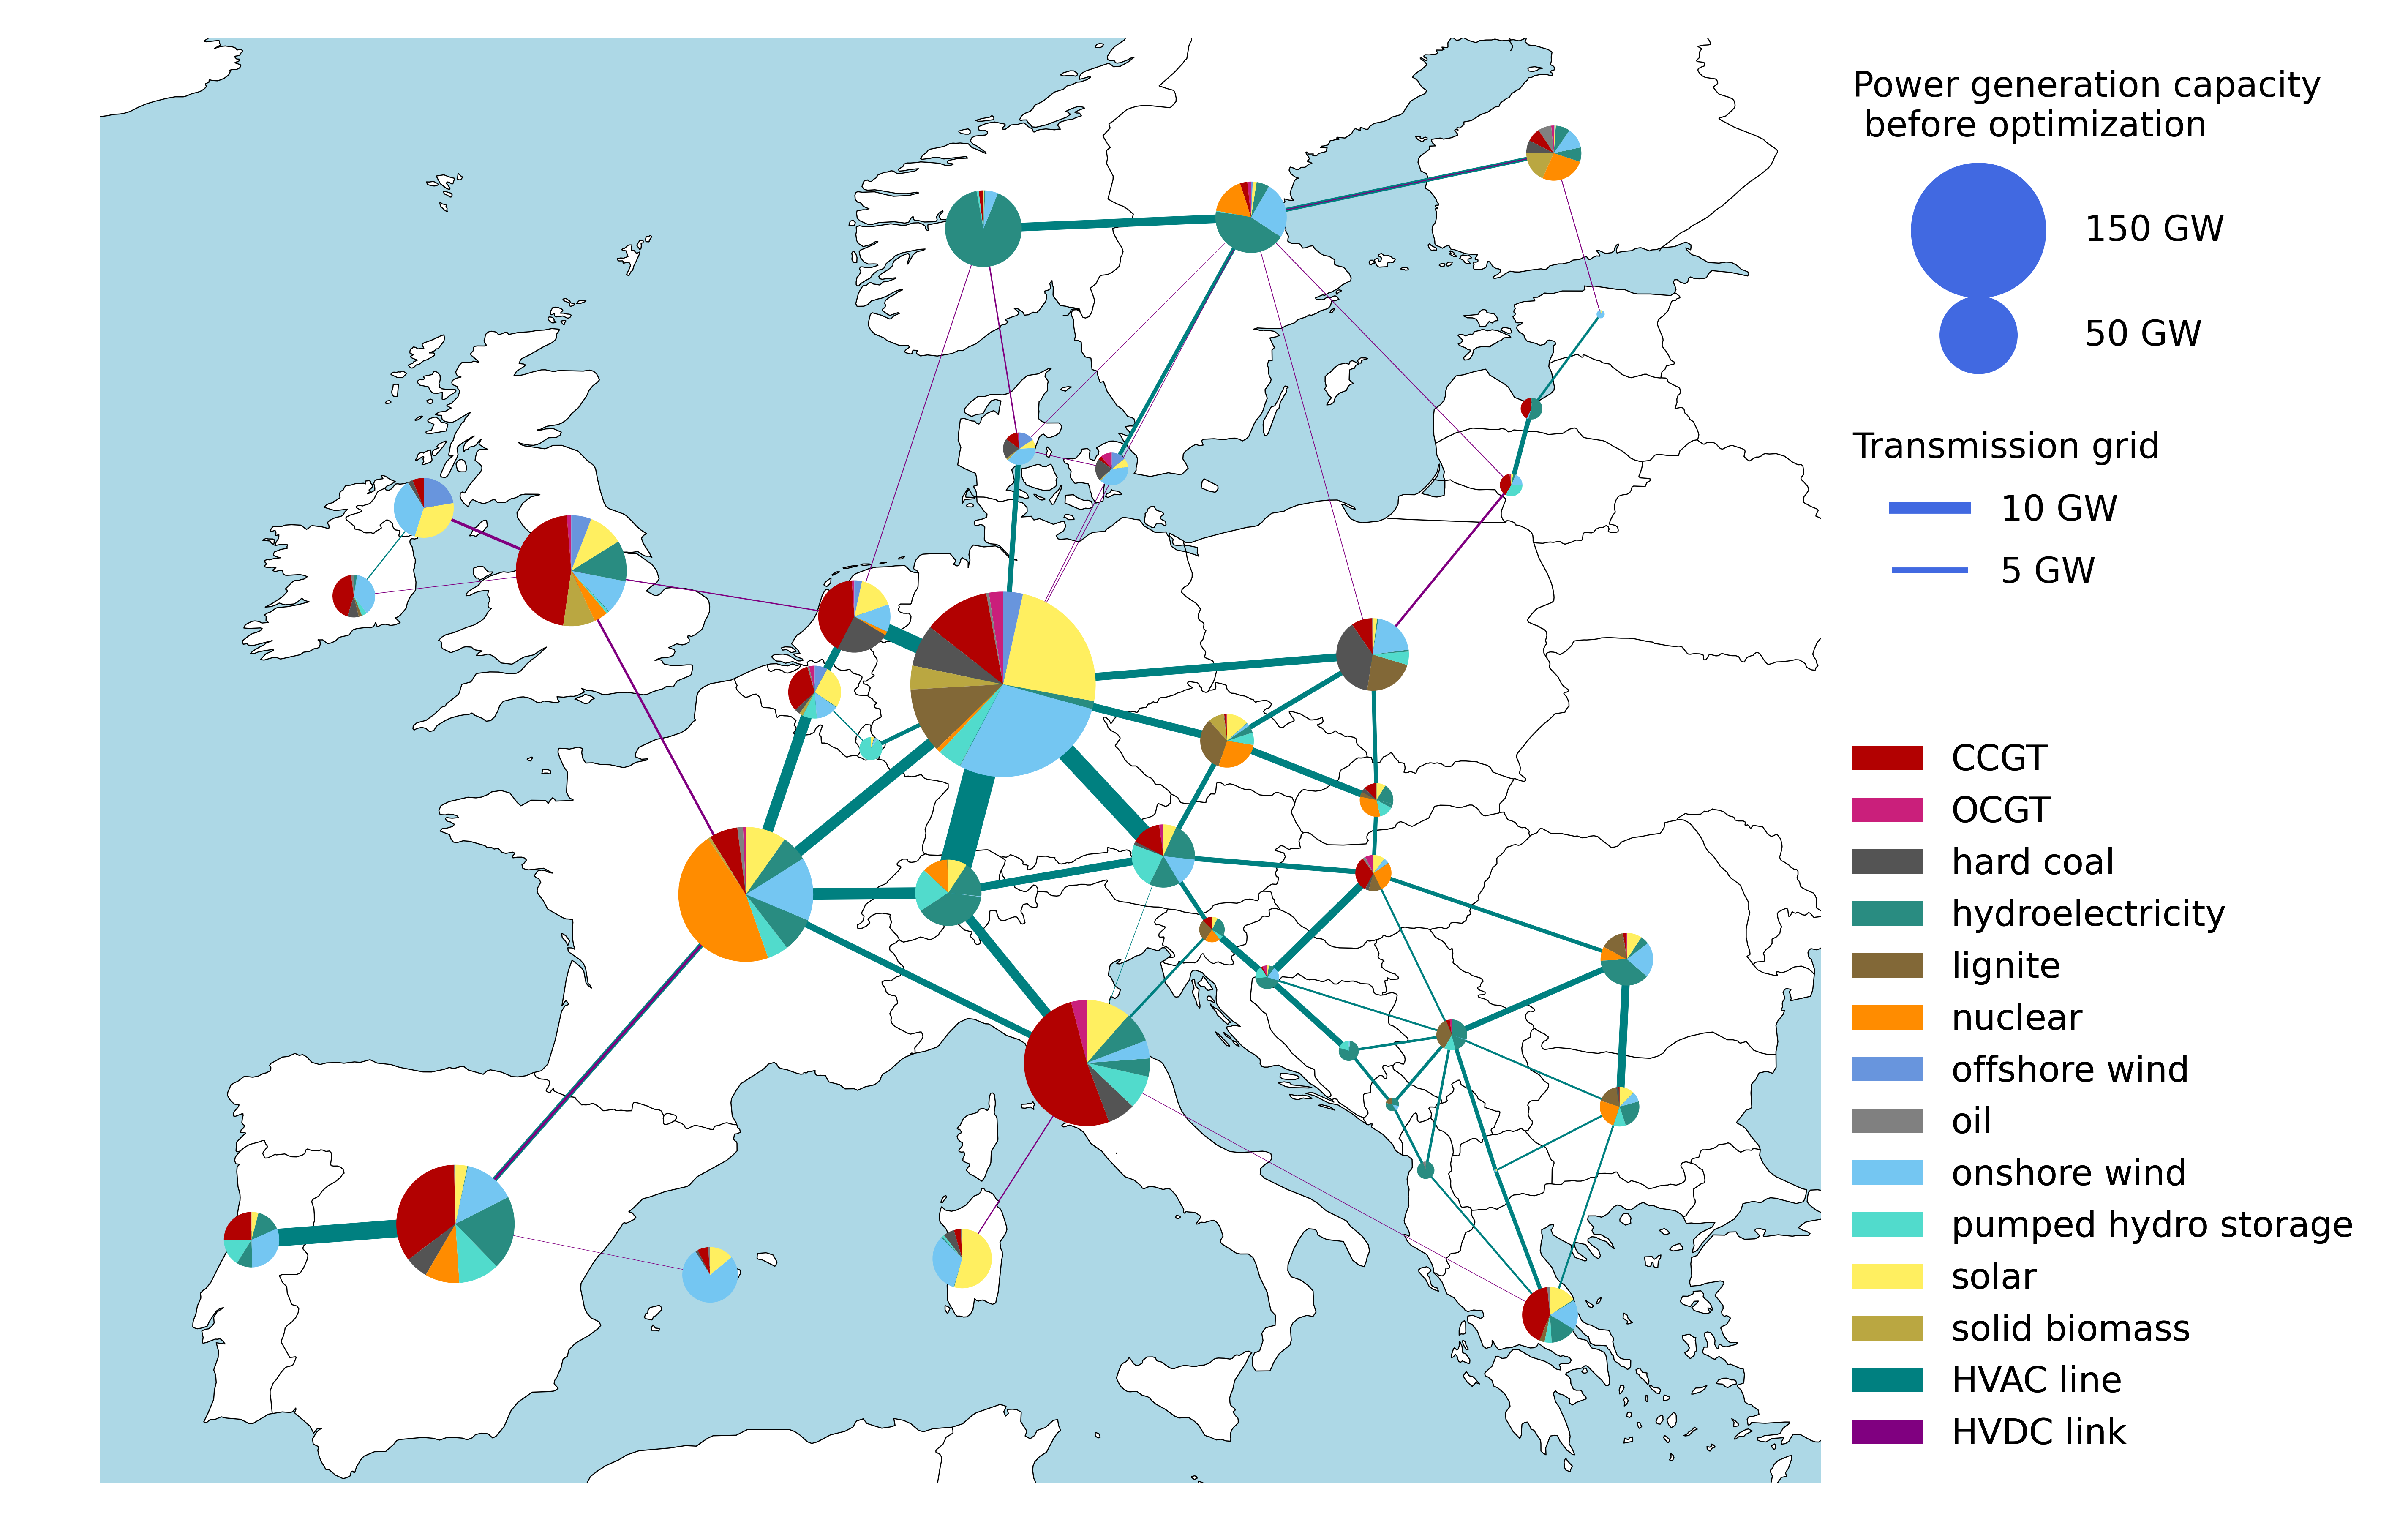
\includegraphics[width=7.5cm]{images/map-fleet.pdf}
  {\scriptsize   PyPSA-Eur network clustered to 37 zones \\ 
  NB power generation capacity fleet before optimization stage}
  \end{column}

  \begin{column}{8cm}
  \begin{itemize}
  \item In each scenario, we model the full European power system (ENTSO-E area) 
  clustered to \alert{37~zones}.

  \item Each zone represents an individual country. Some countries
  that straddle different synchronous areas are split to individual bidding zones, 
  such as DK1 (West) and DK2 (East).

  \item The model \alert{co-optimizes} investment and dispatch decisions of generation \& storage assets to meet electricity demand of data centers (flexible 24/7~CFE consumers), as well as investment and dispatch decisions of assets in the rest of the European electricity system to meet the demand of other consumers. 

  \item All model runs are done with \alert{hourly resolution}, i.e., no time sampling.
  
  \end{itemize}

  \end{column}
  \end{columns}
  }

\end{frame}



\begin{frame}{Study design: data center locations}
  
  {\footnotesize
  \begin{columns}[T]

  \begin{column}{7cm}
  \centering
  \vspace{0.5cm}
  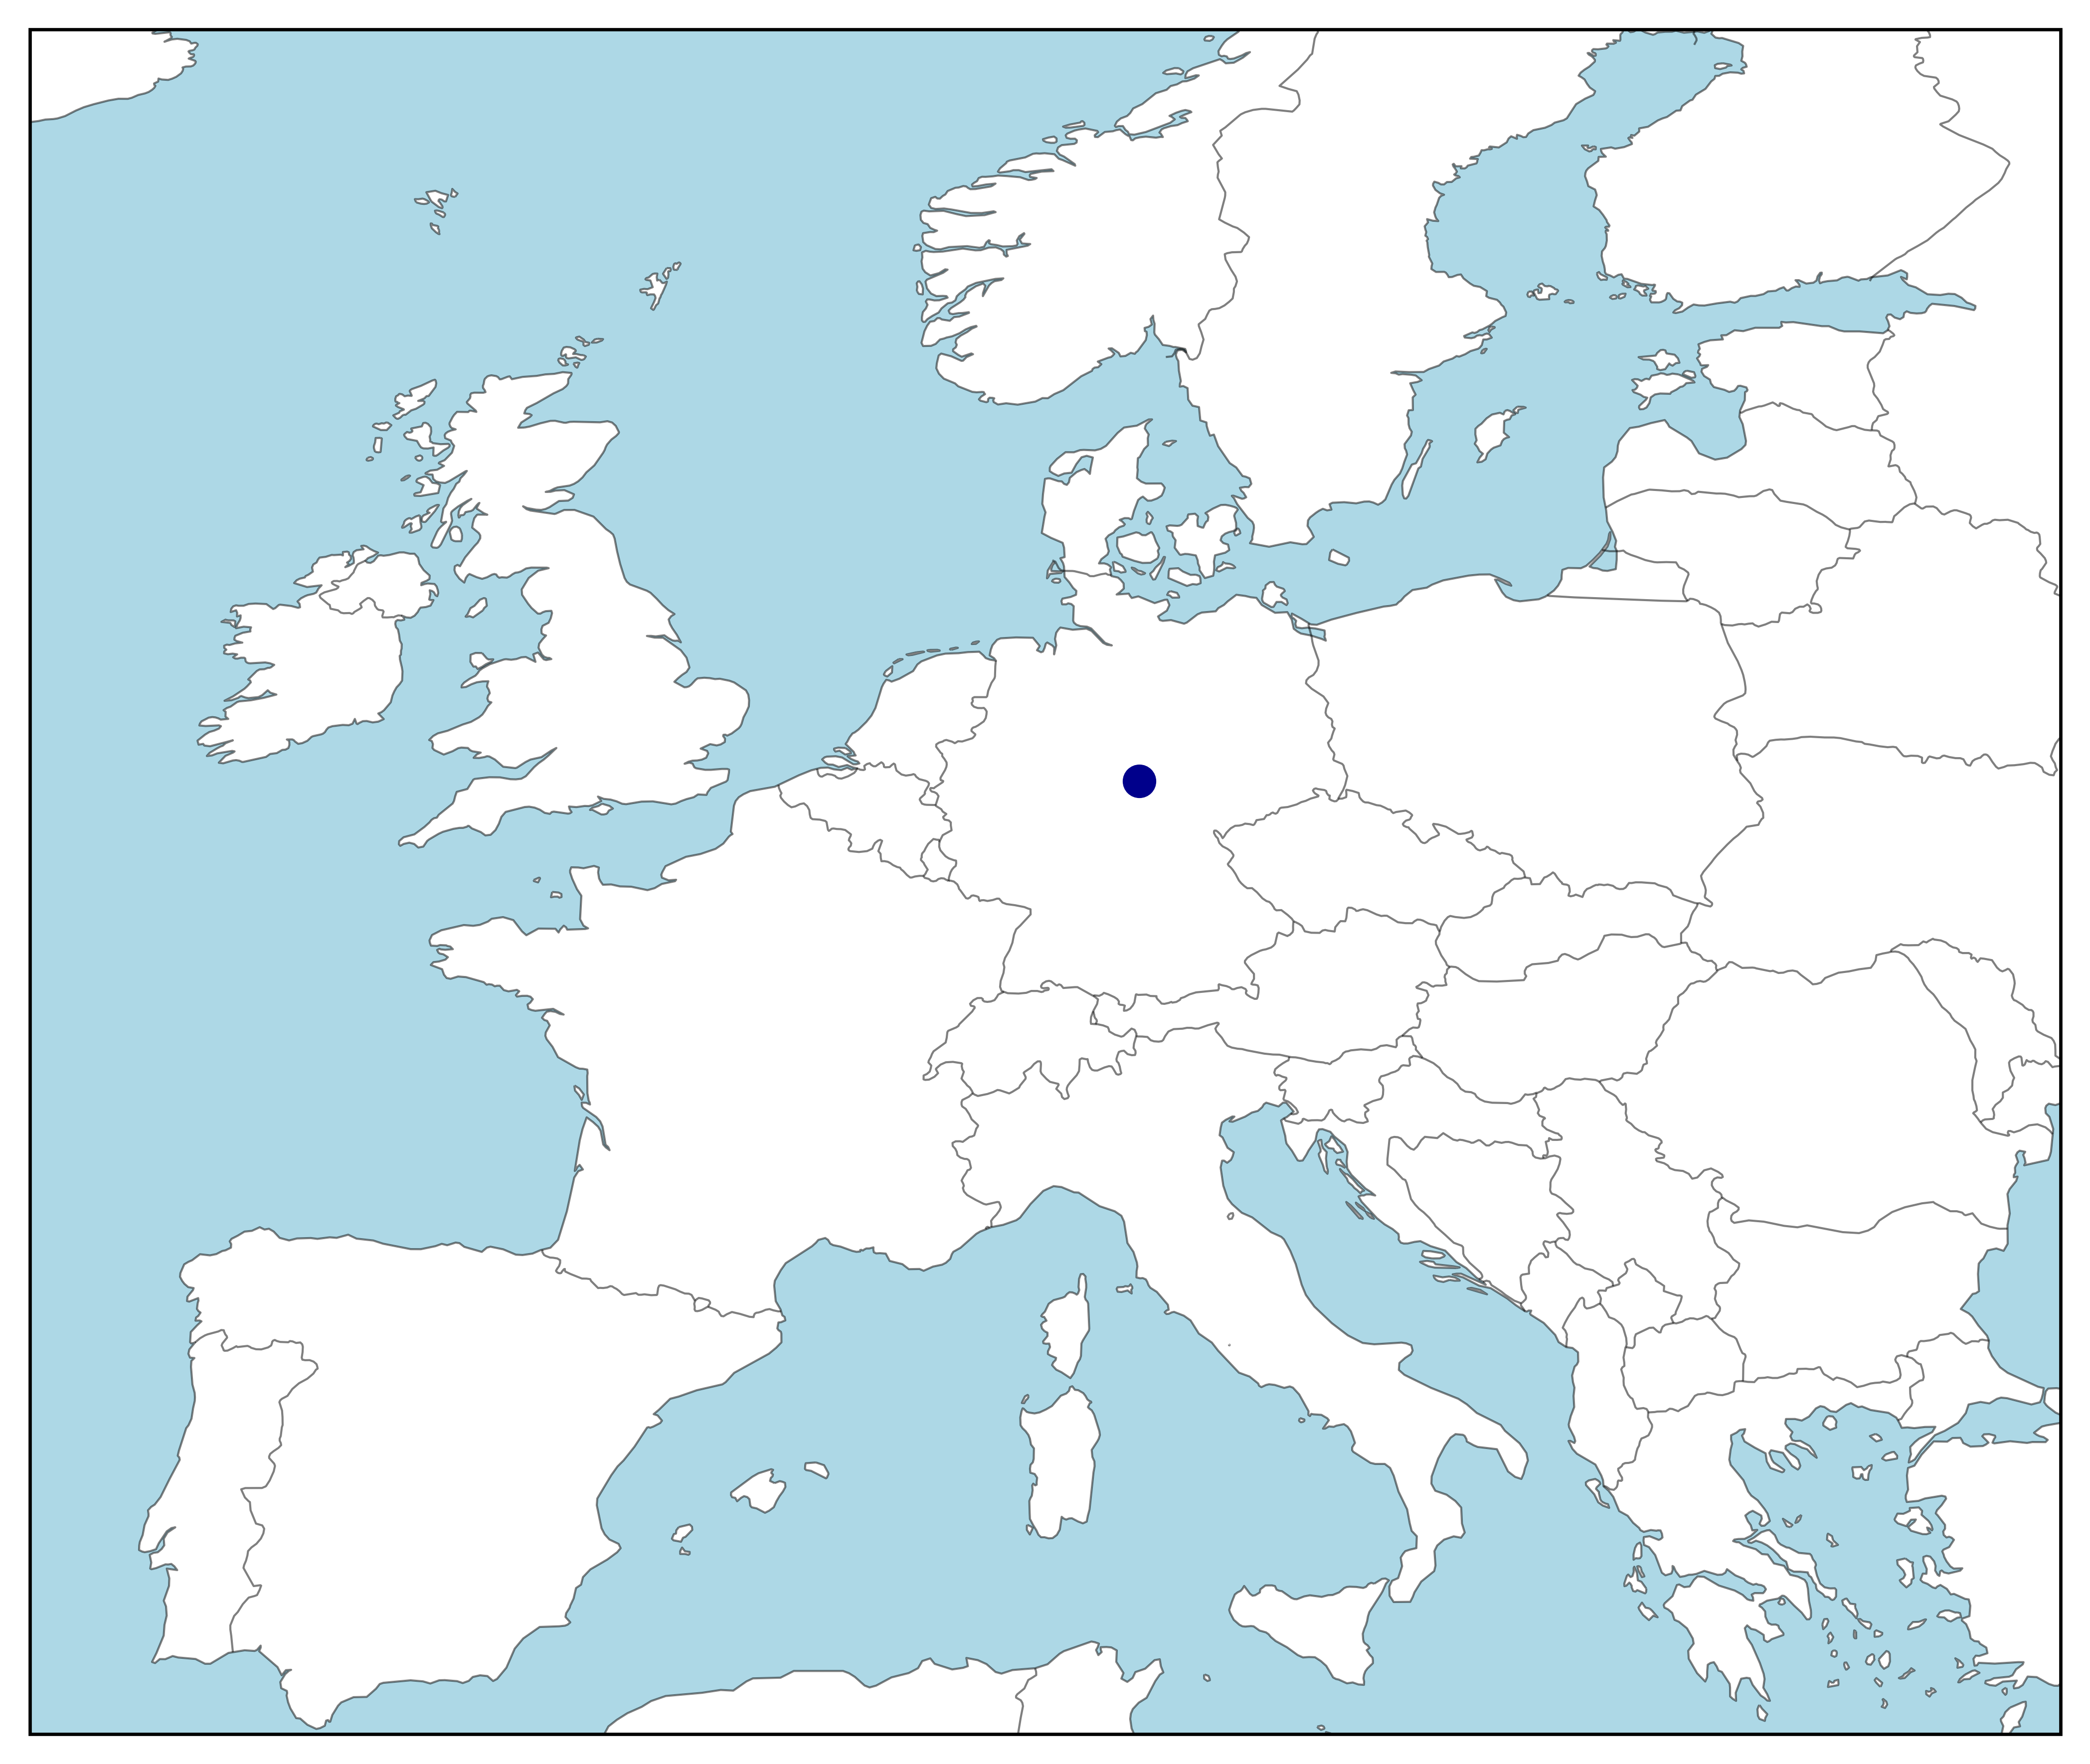
\includegraphics[width=7cm]{images/map-DCs.pdf}
  {\scriptsize Five data centers interconnected by virtual links, \\ 
  forming a complete graph}
  \end{column}

  \begin{column}{8cm}
  \begin{itemize}
    \item We consider \alert{five data centers} that are located in Ireland, Denmark (West/DK1), Germany, Finland, and Portugal. These locations (i) include zones where data centers have an important share in national electricity demand [\hrefc{https://www.statista.com/statistics/878621/european-data-centers-by-country/}{1},\hrefc{https://backend.orbit.dtu.dk/ws/portalfiles/portal/236202284/The_role_of_data_centres_in_the_future_DES_clean_version.pdf}{2},\hrefc{https://www.cso.ie/en/releasesandpublications/ep/p-dcmec/datacentresmeteredelectricityconsumption2021/keyfindings/}{3}], and (ii) each zone has an electricity system with a unique set of characteristics, such as local generation mix, renewable potentials, national energy and climate policies, degree of interconnections, etc. 
    \item Data centers have a nominal load of \alert{100~MW} (baseload profile).
    \item Data center operator aims to achieve a \alert{given 24/7~CFE matching score} at all locations. 
    \item Data centers are interconnected by virtual links, forming a \alert{complete graph} (every pair is connected by a unique virtual link).
    \item Data centers have the \alert{same share of flexible workloads}. 
  \end{itemize}

  \end{column}
  \end{columns}
  }

\end{frame}



\begin{frame}{Study design: scenario space}

  {\footnotesize 
  \begin{itemize}

  \item We model various scenarios for data center demand flexibility, which include \\
  \vspace{0.1cm}
  Three modes of operation: \\
    -- Co-optimized \alert{spatial and temporal} load management \\
    -- Isolated \alert{spatial} load management (shifting flexible workloads across locations)\\ 
    -- Isolated \alert{temporal} load management (shifting flexible workloads in time) \\ 
  \vspace{0.1cm}
  and four scenarios for flexible workloads range: \alert{$f$ = \{0\%, 10\%, 20\%, 40\%\}}.

  \item Three scenarios for 24/7~CFE hourly matching targets:
  \alert{$CFE scores$ = \{90\%, 98\% and 100\%\}}.
  
  \item Further, we assume two palettes of carbon-free technologies available for procurement for data center operators participating in 24/7-CFE: \\
  \vspace{0.1cm}
  -- \alert{Palette~1} includes technologies available on the European market now: onshore wind, utility scale solar PV, battery storage. \\
  -- \alert{Palette~2} includes all above plus Long Duration Energy Storage (LDES) in a form of a hydrogen storage system that is expected to be available for a commercial scale up in the near future. 

  \item For interested parties, we publish an \faLink~\hrefc{tba}{online annex} with a full pack of modelling results alongside this study. The annex includes modelling results for all scenario combinations in a form of plots and summary csv files. 
  % \item We focus on two periods: \alert{2025} and \alert{2030}. The two periods differ by \\ 
  % (i) Technology cost assumptions, \\
  % (ii) National renewable expansion pathways,\\
  % (iii) Power plant fleet (changes take place due to decommissioning based on generators' 
  % age or national policies), \\
  % (iv) System-wide assumptions, such as price for EU ETS allowances.

  \end{itemize}
  }
\end{frame}



\begin{frame}{Study design: limitations}
  
  {\footnotesize 
  \begin{itemize}

  \item This study is done in a spirit of \alert{modelling for insight} rather than \alert{modelling for numbers}. The design of this study does not aim at quantifying the real-life benefits of demand side flexibility for data centers. It is rather a model experiment to explore \textit{why and how} flexibility of demand can be beneficial for achiving 24/7 carbon-free energy goals. The results we present can thus be viewed with a fair degree of caution, i.e., as a modelling-based insights rather than quantitative projections for the future. 
  
  \item Quantifying the actual costs benefits for the ICT industry of utilising demand flexibility requires \alert{additional empirical research}. Further studies could usefully explore the costs of achieving a certain share of flexible workloads beared by data center operators, which are not considered in this study. Including information on implicit flexibility costs would help to quantify the flexibility benefits with a greater degree of accuracy. Another empirical improvement could address technical aspects and properties of flexible workloads, such as physical constraints associated with quick ramping of power usage up/down, safety constraints, etc.
  
  \end{itemize}
  }
  \end{frame}


%----------------------------------------
%----------------------------------------
\section{Data sources and assumptions}


\begin{frame}{Data sources: electricity grid}
 
  \begin{columns}[T]
  \begin{column}{6cm}

  \centering

  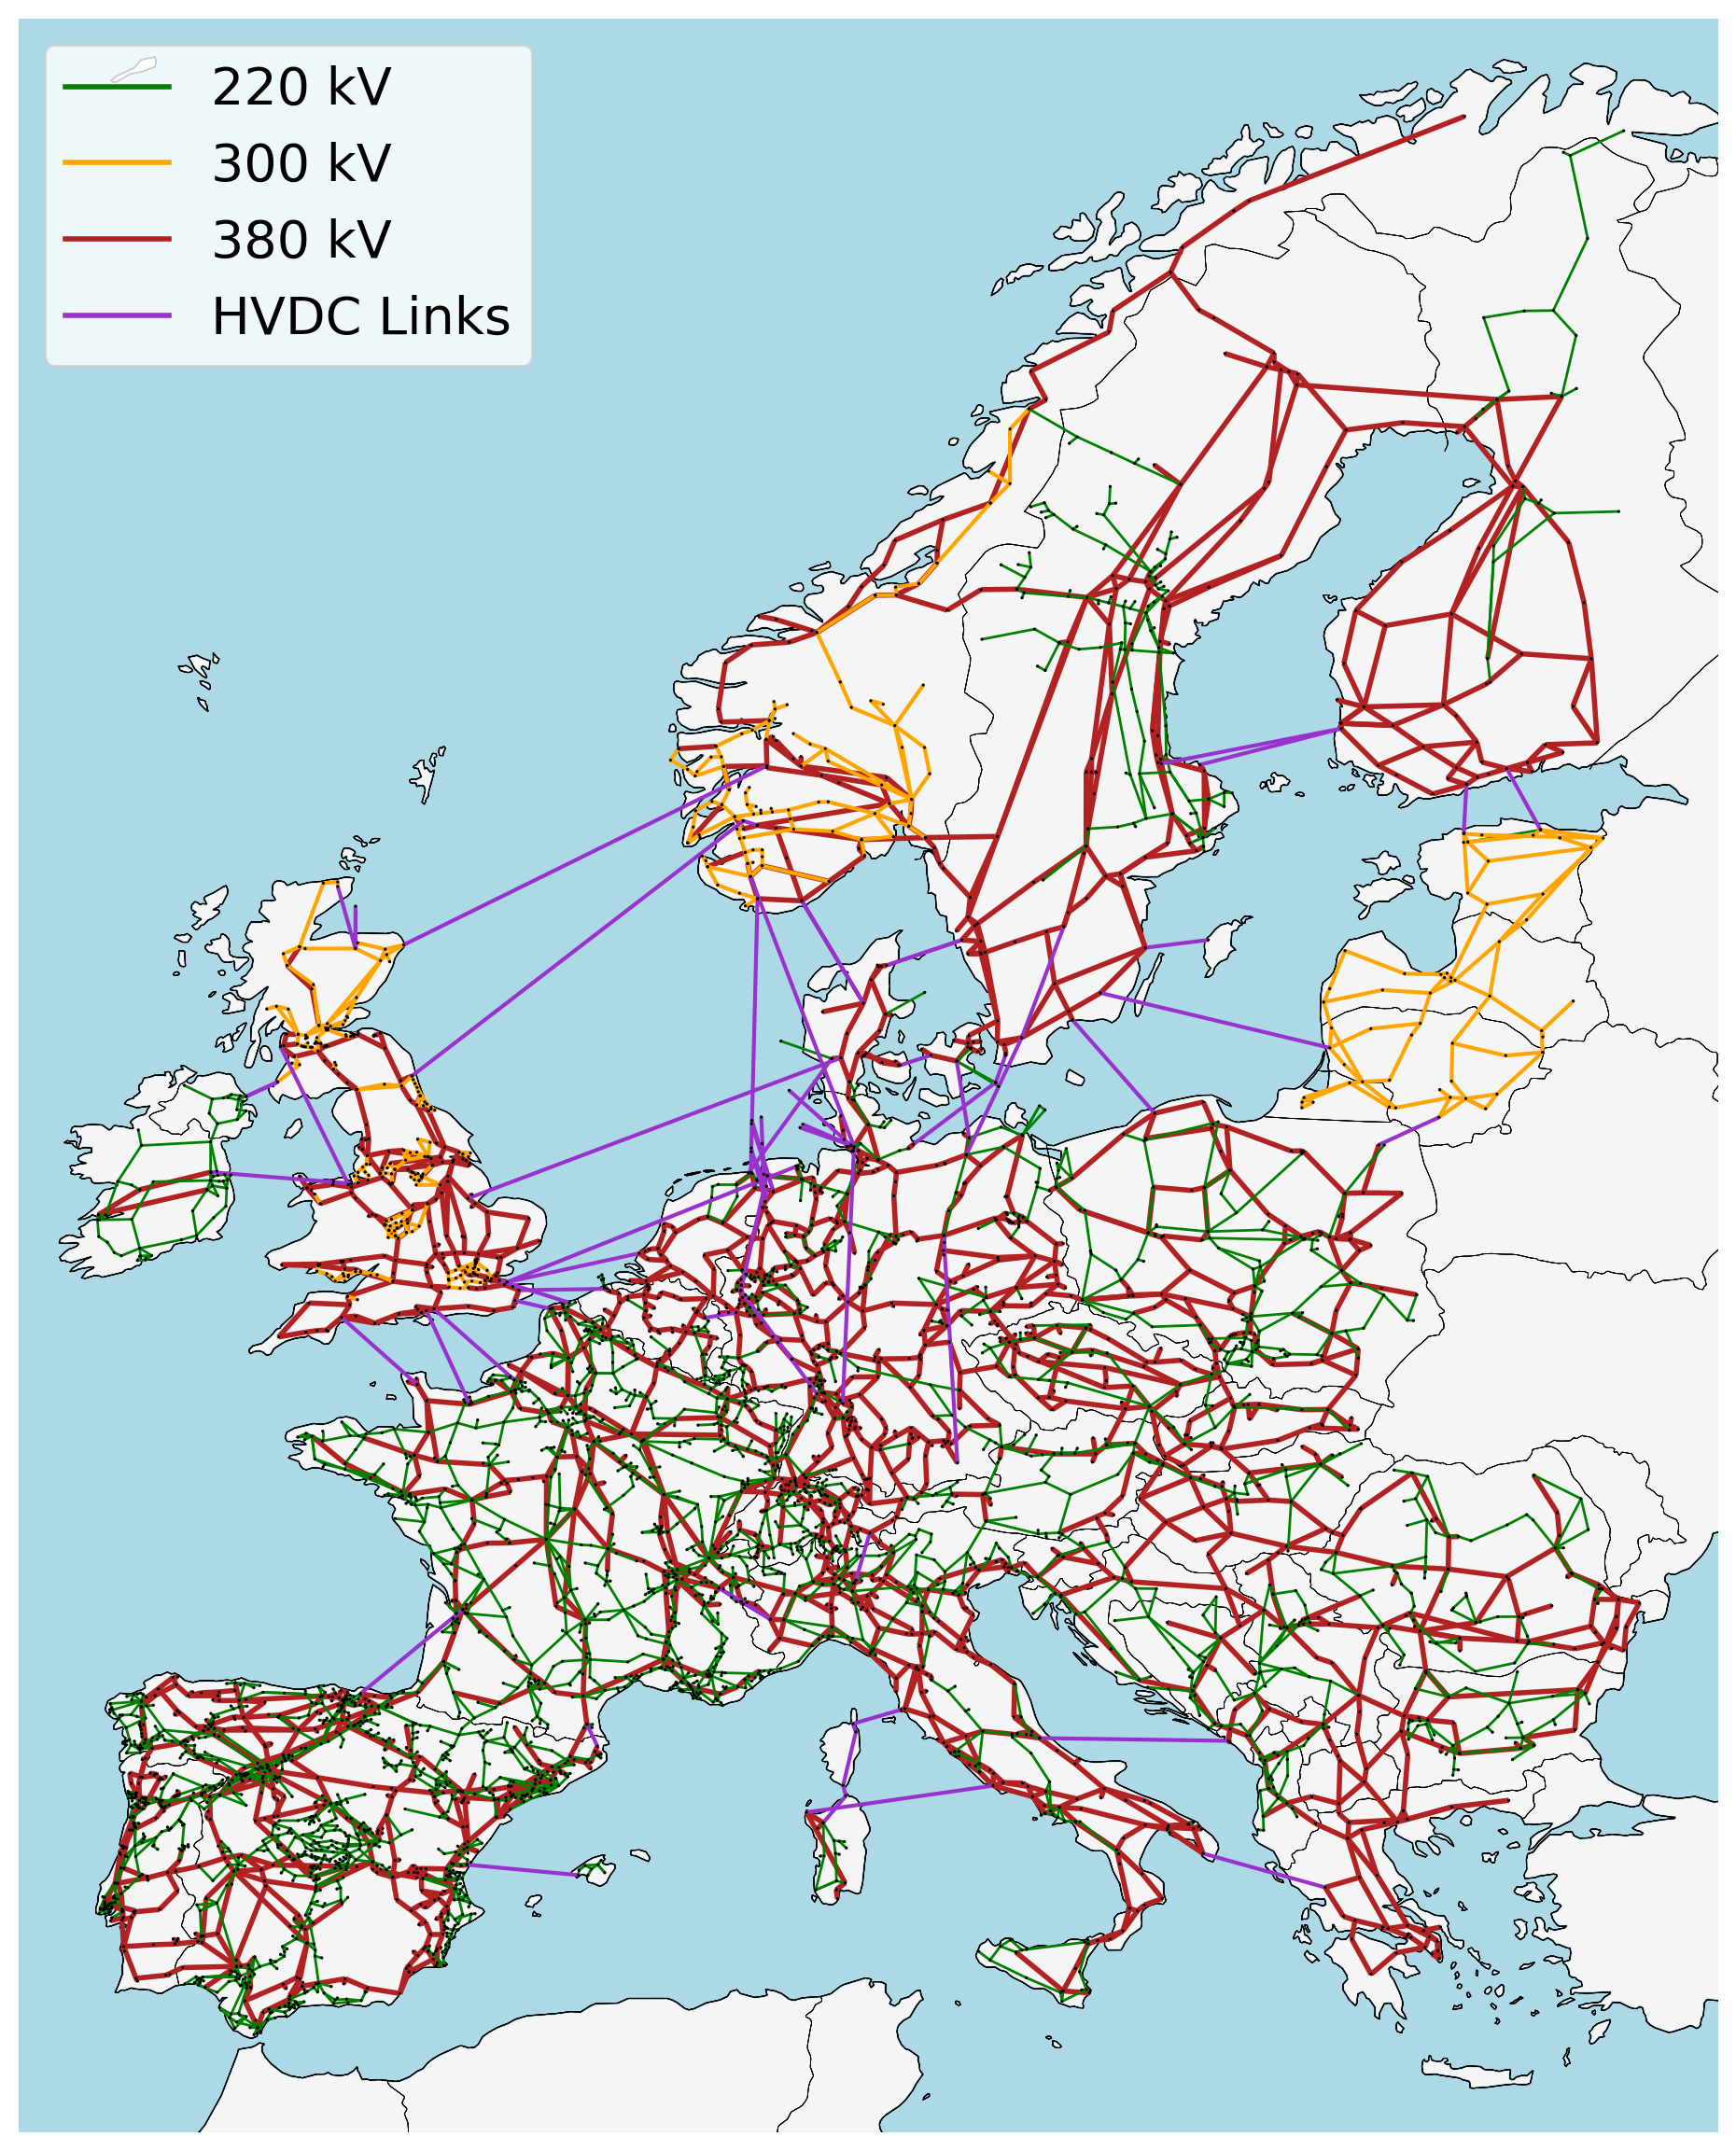
\includegraphics[width=6.5cm]{images/pypsa-eur-grid.png}

  {\footnotesize 
  \vspace{.1cm}
  Basic validation of grid model in 
  \hrefc{https://doi.org/10.1016/j.esr.2018.08.012}{Hörsch et al. (2018)}
  }
  \end{column}

  \begin{column}{9cm}
  {\small 
  \begin{itemize}
    \item Grid data contains AC lines at and above 220~kV voltage level, 
    all high voltage DC lines, and substations for the full 
    \hrefc{https://www.entsoe.eu/data/map/}{ENTSO-E area}.
    \item Grid data is collected by a modified \faGithub~\hrefc{https://github.com/PyPSA/GridKit}{GridKit} extraction of the \hrefc{https://www.entsoe.eu/data/map/}{ENTSO-E Transmission System Map}. GridKit uses spatial and topological analysis to transform map objects from the ENTSO-E interactive map into a network model of the electric power system. The full grid model contains near 6760 lines and 3640 substations. 
    \item The number of nodes fed into optimization model is adjustable, what allows for spatial and topological analysis at 
    \hrefc{https://pypsa-eur.readthedocs.io/en/latest/spatial_resolution.html}{different levels}. The number of nodes can vary between 37 (the number of independent countries / synchronous areas) and several hundred (for computational tractability).\\
  \end{itemize}
  }
  
  \end{column}
  \end{columns}

  \source{Image: \href{https://github.com/PyPSA/pypsa-eur}{github.com/PyPSA/pypsa-eur}}
\end{frame}



\begin{frame}{Data sources: power plants}
 
  \begin{columns}[T]\

  \begin{column}{8cm}
    {\small 
    \begin{itemize}
      \item Existing power generation fleet data is collected with a \href{https://github.com/PyPSA/powerplantmatching}{\alert{powerplantmatching}} toolset.
      
      \item Powerplantmatching cleans, standardizes and merges the data from multiple open \hrefc{https://powerplantmatching.readthedocs.io/en/latest/basics.html}{power plant datasets} to create a combined dataset, which includes all the important information about power plants in Europe in a ready-to-use format for energy system modelling. 
      
      \item The toolset allows to update the combined data as soon as new input datasets are released.
  
      \item Powerplantmatching is an open-source project maintained by TU Berlin team. \\
      \faGithub~\hrefc{https://github.com/PyPSA/powerplantmatching}{GitHub} \\
      \faBook~\hrefc{https://powerplantmatching.readthedocs.io/en/latest/index.html}{Documentation}
    
    \end{itemize}
    }  
  \end{column}

  \begin{column}{7cm}
  \vspace{0.5cm}
  \centering
  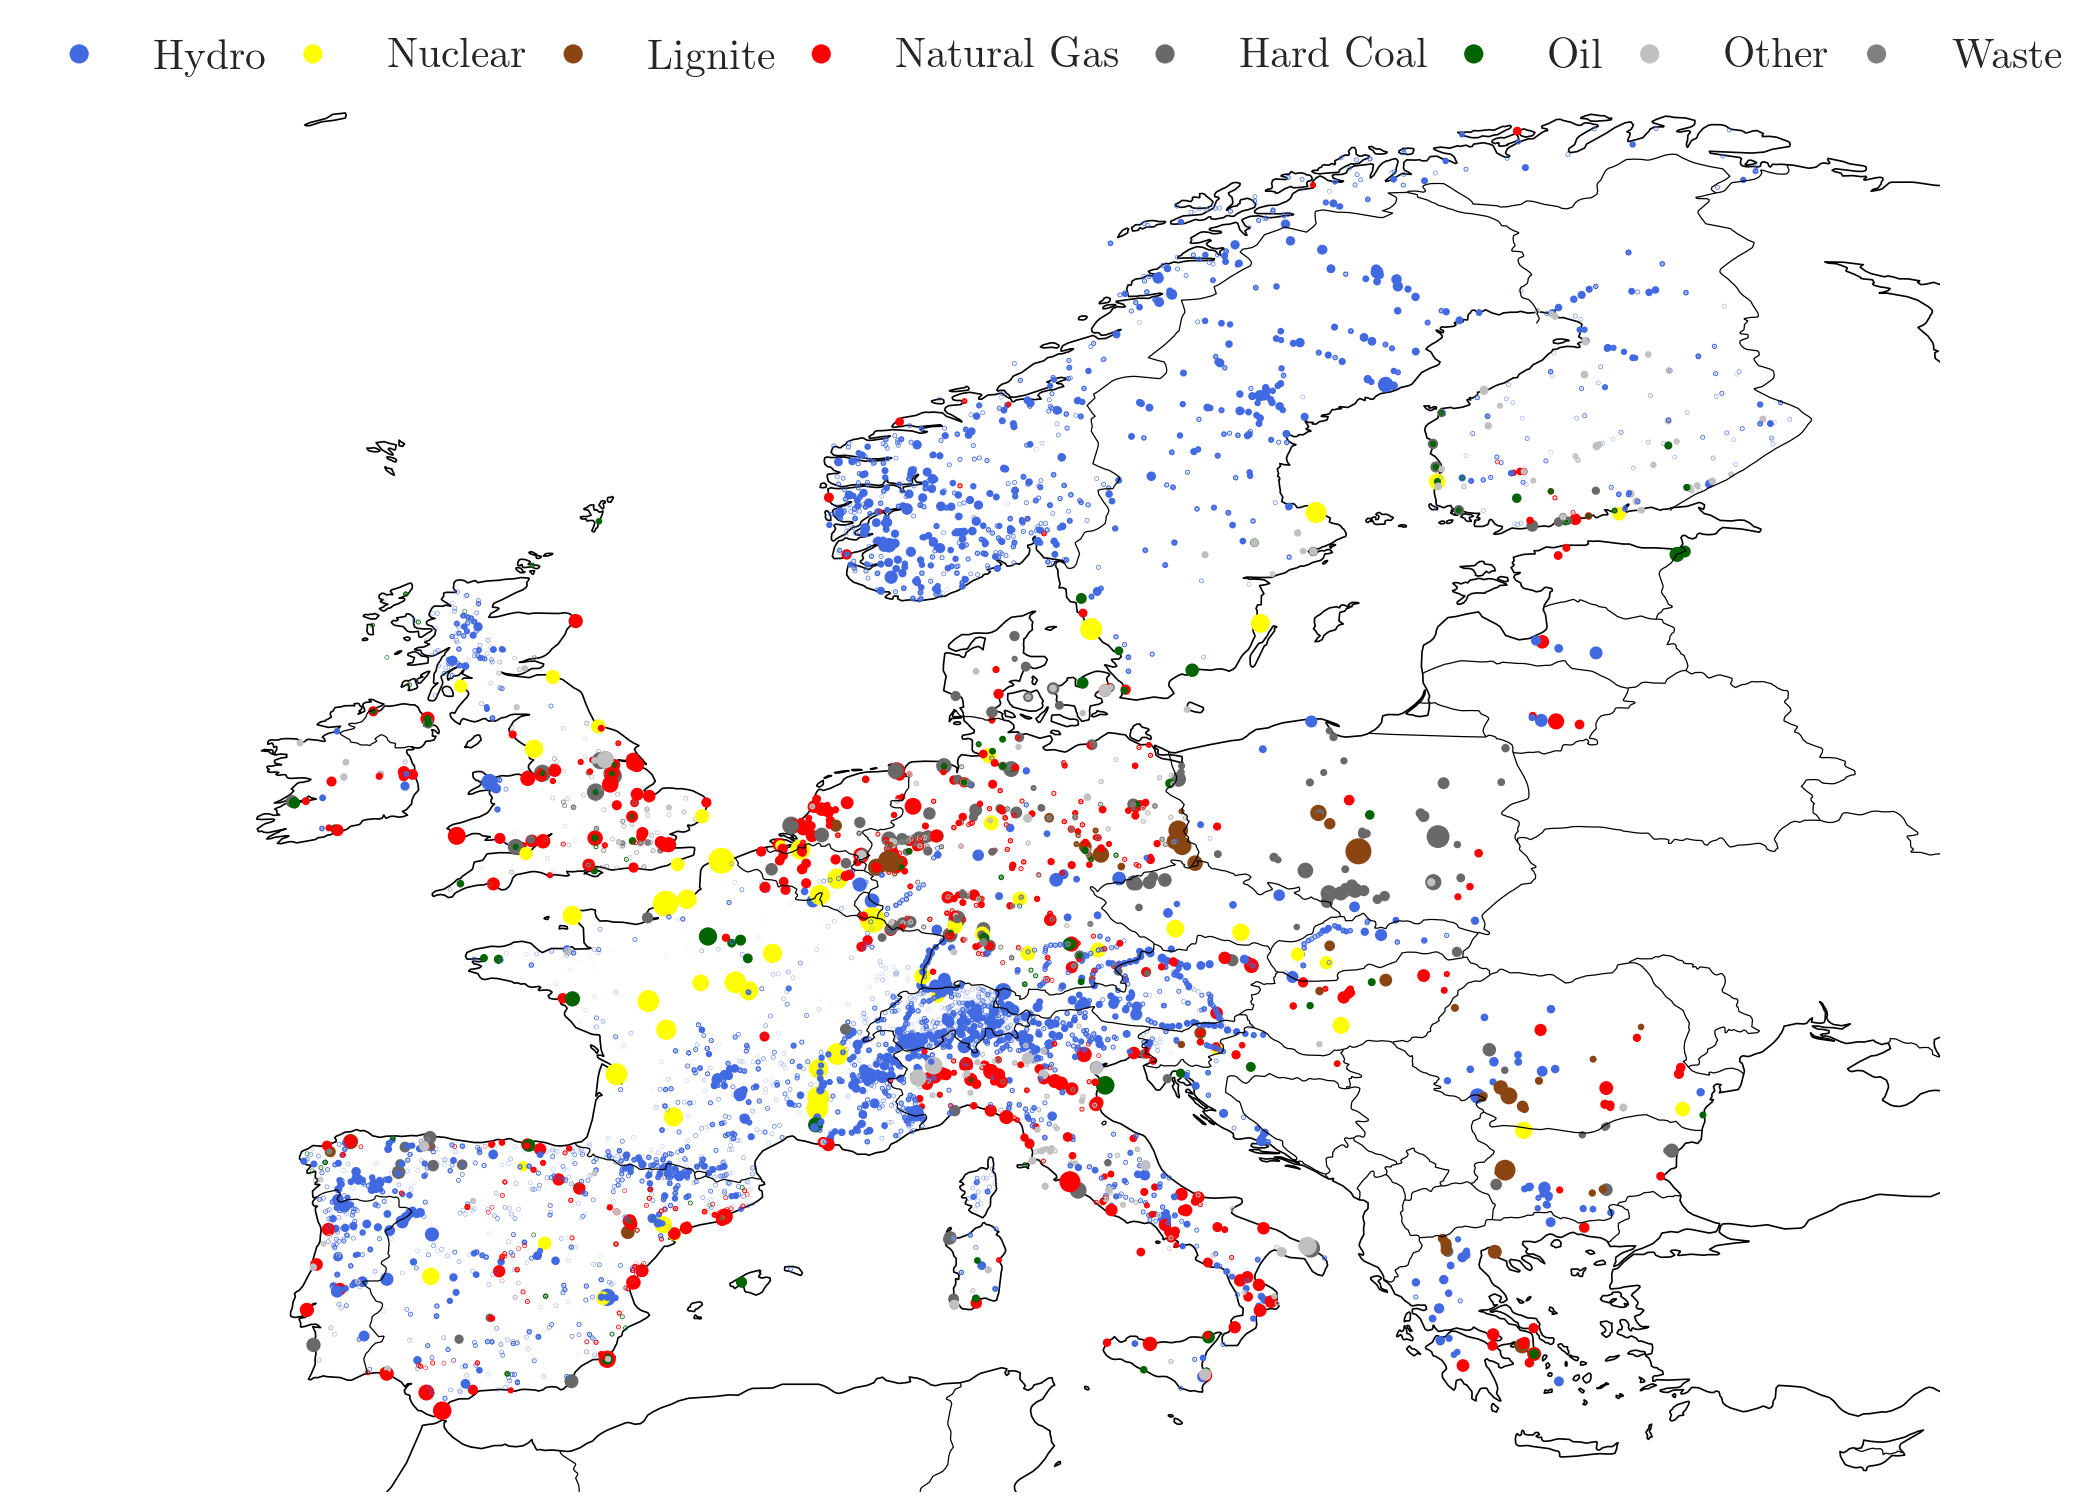
\includegraphics[width=7.2cm]{images/powerplantmatching.png}
  \end{column}

  \end{columns}
  \source{Image: \href{https://github.com/PyPSA/powerplantmatching}{github.com/PyPSA/powerplantmatching}}

\end{frame}



\begin{frame}{Data sources: technology cost assumptions}
 
  \begin{columns}[T]\

  \begin{column}{8cm}
    {\small 
    \begin{itemize}
      \item The database of assumptions for energy system technologies (such as capital and operational costs, efficiencies, lifetimes, etc.) is retrieved from the repository \alert{\href{https://github.com/pypsa/technology-data}{PyPSA/technology-data}}. 
      
      \item The technology-data project compiles information about energy technologies from a variety of sources. The complied dataset has standardized technology names and energy units. All values are linked to original sources.

      \item  technology-data is an open-source project maintained by TU Berlin team. \\
      \faGithub~\hrefc{https://github.com/PyPSA/technology-data}{GitHub} \\
      \faBook~\hrefc{https://technology-data.readthedocs.io/en/latest/}{Documentation}

    \end{itemize}}  
  \end{column}

  \begin{column}{7cm}
  \centering
  
\includegraphics[width=7.2cm]{images/technology-data.png}
  \vspace{0.5cm}
  {\small
  \begin{flushright}
    Cost assumptions used in this study originate from the \hrefc{https://ens.dk/en/our-services/projections-and-models/technology-data}{technology data catalogue} published by The~Danish~Energy~Agency.
  \end{flushright}
  }
  \end{column}
  \end{columns}

  \source{Image: \href{https://github.com/PyPSA/technology-data}{github.com/PyPSA/technology-data}}
\end{frame}



\begin{frame}{Data sources: renewable potentials and time series}
 
  \begin{columns}[T]
  \begin{column}{8cm}

  \vspace{0.5cm}
  \centering

  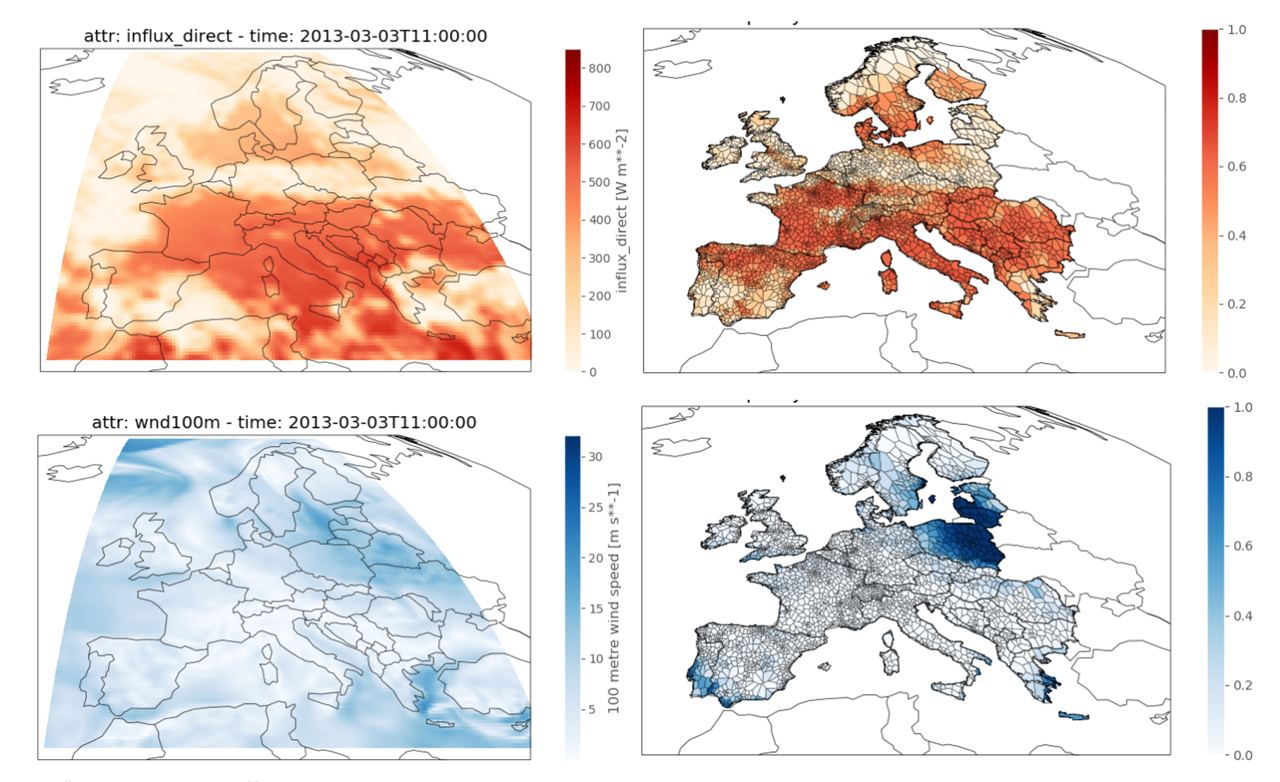
\includegraphics[width=8cm]{images/atlite.jpg}

  {\footnotesize 
  Converting weather data to energy system data
  }
  \end{column}

  \begin{column}{8cm}
  \vspace{-0.2cm}
  {\small 
  \begin{itemize}
    \item Renewable power potentials and generation profiles are processed by 
    the \href{https://github.com/PyPSA/atlite}{\alert{atlite}} package, 
    which converts terabytes of weather data (like wind speeds, solar influx) 
    into the data for energy systems modelling.
    \item With atlite, we process datasets for land cover (CORINE2018), natural protection areas (NATURA2000), and bathymetry (GEBCO2018) to conduct own geospatial land availability analysis.\\The standard data source for renewable time time-series estimation is ECMWF's ERA5 dataset (reanalysis weather data in ca. 30km x 30km and hourly resolution). 
    \item  atlite is also an open-source project maintained by TU~Berlin team. \\
    \faGithub~\hrefc{https://github.com/PyPSA/atlite}{GitHub} \\
    \faBook~\hrefc{https://atlite.readthedocs.io/en/latest/}{Documentation}

  \end{itemize}
  }
  \end{column}
  \end{columns}

\source{Image: \href{https://github.com/PyPSA/atlite}{atlite.readthedocs.io/}}
\end{frame}



\begin{frame}{Other background system assumptions}

\begin{itemize}
  {\small 
\item Electrical demand time-series is based on the 
\hrefc{https://open-power-system-data.org/}{OPSD project}. 
We assume the same demand profile per bidding zone for 2025 and 2030, as in the representative year 2013. 
\item We assume 2013 as the representative climate year for renewable in-feed.
\item Renewable expansion in the background electricity system is endogenous; we implement renewable generation targets by country that follow the \hrefc{https://energy.ec.europa.eu/topics/energy-strategy/national-energy-and-climate-plans-necps_en}{national energy and climate plans}. For countries w/o a 2025 target, a linear increase from renewable generation in 2020 to 2030 target is assumed. The modelled \co~emission intensity of electricity generation in European energy system matches the \hrefc{https://www.eea.europa.eu/ims/greenhouse-gas-emission-intensity-of-1}{estimated values} for 2025/2030.
\item  National policies and decommissioning plans for coal and nuclear 
power plants are based on the 
\hrefc{https://beyond-coal.eu/}{Europe Beyond Coal}, 
and \hrefc{https://world-nuclear.org/}{world-nuclear.org} projects.
\item We assume price for EU ETS allowances to be 80~\euro/tCO$_2$ 
and 130~\euro/tCO$_2$ for 2025 and 2030, accordingly.\footnote{{\scriptsize 
Based on estimates of \hrefc{https://doi.org/10.1016/j.apenergy.2021.116914}{Pietzcker et al. 2021}
}}
The price for natural gas is assumed to be 35~\euro/MWh.\footnote{{\scriptsize Based on the price assumptions in the \hrefc{https://energy.ec.europa.eu/system/files/2022-05/SWD_2022_230_1_EN_autre_document_travail_service_part1_v3.pdf}{REPowerEU Plan}
issued by the European Commission in May 2022}}
}
\vspace{0.2cm}
\end{itemize}

\end{frame}


\begin{frame}{Assumptions about technologies available for 24/7~CFE consumers}
  
  \centering
  {\footnotesize 

    \begin{tabular}{cccccccc}
      \hline
      \hline
      Year & Technology & CAPEX & FOM & VOM & Efficiency & lifetime \\
       &  & (overnight cost)  &  (\%/year) &  (€/MWh) & (per unit) & (years) \\
      \hline
      \hline
      2025 & utility solar PV & 612 €/kW & 1.7 & 0.01 & - & 37.5 \\
      \hline
      2025 & onshore wind & 1077 €/kW & 1.2 & 0.015 & - & 28.5 \\
      \hline
      2025 & battery storage & 187 €/kWh & 0 & - & - & 22.5 \\
      \hline
      2025  & battery inverter & 215 €/kW & 0.3 & - & 0.96  & 10.0 \\
      \hline
      2025 & hydrogen storage\footnote{{\scriptsize Underground hydrogen storage in salt cavern}} 
                  & 2.5 €/kWh & 0 & - & - & 100.0 \\
      \hline
      2025 & electrolysis & 550 €/kW & 2.0 & - & 0.67 & 27.5  \\
      \hline
      2025 & fuel cell & 1200 €/kW & 5.0 & - & 0.50 & 10.0 \\
      \hline
      \hline
      2030 & utility solar PV & 492 €/kW & 2.0 & 0.01 & - & 40.0 \\
      \hline
      2030 & onshore wind & 1035 €/kW & 1.2 & 0.015 & - & 30 \\
      \hline
      2030 & battery storage & 142 €/kWh & 0 & - & - & 25 \\
      \hline
      2030  & battery inverter & 160 €/kW & 0.3 & - & 0.96  & 10.0 \\
      \hline
      2030 & hydrogen storage  & 2.0 €/kWh & 0 & - & - & 100.0 \\
      \hline
      2030 & electrolysis & 450 €/kW & 2.0 & - & 0.68 & 30  \\
      \hline
      2030 & fuel cell & 1100 €/kW & 5.0 & - & 0.50 & 10.0 \\
      \hline
      \hline
      \end{tabular}
  
    Data is originally retrieved from the \hrefc{https://ens.dk/en/our-services/projections-and-models/technology-data}{DEA's catalogue for energy technologies}
      \vspace{0.2cm}
  }
\end{frame}



%---------------------------------------------
%---------------------------------------------
\section{Modelling results and analysis}


%----------------------------------

\begin{frame}{Base scenario: Ireland -- Palette 1}

{\footnotesize
\vspace{0.3cm}

\begin{columns}[T]
\begin{column}{9cm}
\centering

\includegraphics[width=9.4cm]{../results/report/plots/10/2025/IE/p1/ci_emisrate.pdf}

\end{column}
\begin{column}{6cm}

\vspace{0.1cm}
Next, we investigate how the choice of a procurement policy affects the {\bf average emissions 
rate} of 24/7 participating C\&I consumers.

\vspace{0.3cm}
Already in 2025, Ireland has a moderately clean electricity system: 
the C\&I emission rate in the reference case is at 138~kg/MWh.

\vspace{0.3cm}
100\% annual matching with renewable energy reduces the 
C\&I emission rate to 53 kg/MWh.

\vspace{0.3cm}
When actively matching the carbon-free electricity and the load with 
24/7 procurement, C\&I participants can achieve \alert{lower emission 
rates than with the 100\% RES policy} with CFE targets beyond 85\%. 
As CFE target is tightened further, average emissions \alert{drop to zero}.

\end{column}
\end{columns}
}
\source{Ireland -- Palette 1 -- 2025 -- 10\% -- baseload}
\end{frame}



\begin{frame}{Base scenario: Ireland -- Palette 1}

  {\footnotesize
  \vspace{0.3cm}
  
  \begin{columns}[T]
  \begin{column}{9cm}
  \centering
  
  \includegraphics[width=9.4cm]{../results/report/plots/10/2025/IE/p1/ci_capacity.pdf}
  \end{column}
  \begin{column}{6cm}
  
  \vspace{0.1cm}
  If we now turn to the {\bf portfolio capacity} procured by 
  C\&I consumers, we see that at this level of participation
  (10\% of C\&I load in Ireland is at 220~MW), the 100\% RES policy can be 
  me by procuring near to 1.5~GW of onshore wind and solar generators.
  
  \vspace{0.3cm}
  In this scenario, hourly matching renewable generation and the 24/7 participating load
  requires a \alert{much bigger portfolio} of renewable generators than the 
  100\% RES policy. 

  \vspace{0.3cm}
  Also, above 85\% 24/7 procurement sees \alert{battery storage} enter the portfolio  mix.
  
  \vspace{0.3cm}
  Note that for 80\% CFE, 24/7 participating C\&I consumers procure less 
  capacity than for 100\% RES policy, as it relies more on grid imports.

  \end{column}
  \end{columns}
  }
  \source{Ireland -- Palette 1 -- 2025 -- 10\% -- baseload}
  \end{frame}



\begin{frame}{Base scenario: Ireland -- Palette 1}

    {\footnotesize
    \vspace{0.3cm}
    
    \begin{columns}[T]
    \begin{column}{9cm}
    \centering
    
    \includegraphics[width=9.4cm]{../results/report/plots/10/2025/IE/p1/ci_costandrev.pdf}
    \end{column}
    \begin{column}{6cm}
    
    \vspace{0.1cm}
    It is also interesting to look at the {\bf breakdown of costs associated with
    a procurement policy} that C\&I consumers choose. 
    
    \vspace{0.3cm}
    Note that revenues from selling the excess electricity to the regional grid 
    (dark green) at market prices can be treated as "negative costs" and 
    subtracted from the net procurement cost.

    \vspace{0.3cm}
    A CFE target of 90-95\% can be achieved at a small cost premium to 100\% 
    annual renewable matching with solar, wind and batteries. However,
    what stands out in the plot is the rapid increase of procurement costs  
    for high CFE targets. For example, 98\% CFE target has 
    cost premium of only 55\% over 100\% annual renewable matching; while
    \alert{the last 2\% of hourly CFE matching more than doubles the 
    cost}.
  
    \end{column}
    \end{columns}
    }
    \source{Ireland -- Palette 1 -- 2025 -- 10\% -- baseload}
    \end{frame}



\begin{frame}{Base scenario: Ireland -- Palette 2}

    {\footnotesize
  
    \begin{columns}
    \begin{column}{7cm}
    \centering
    \includegraphics[width=7.5cm]{../results/report/plots/10/2025/IE/p2/ci_capacity.pdf}
    \end{column}
  
    \begin{column}{8cm}
    \centering
    \includegraphics[width=7.5cm]{../results/report/plots/10/2025/IE/p2/ci_costandrev.pdf}
    \end{column}
  
    \end{columns}
  
    \begin{columns}
    \begin{column}{15cm}
    If we look at the results for the technological {\bf Palette 2} -- 
    when C\&I consumers have an access to the long-duration energy storage (LDES) --
    we see a different picture. The portfolio of renewable capacity 
    C\&I consumers for the 100\% CFE target is not much larger 
    than for 100\% RES (see the left panel). The LDES system helps to align the load 
    with the generation of procured variable renewable resources. 
    In the right panel, we can see that a LDES system (here 2.5~€/kWh 
    hydrogen storage in caverns) can \alert{significantly limit the procurement cost
    increase} at high CFE targets. In this scenario, 
    100\% CFE costs only 50\% more than a 100\% RES policy.

    \end{column}
    \end{columns}
    }
  
    \source{Ireland -- Palette 2 -- 2025 -- 10\% -- baseload}
\end{frame}


%----- base scenario, system effects


\begin{frame}{Base scenario: Ireland -- Palette 3}

  {\footnotesize
  \vspace{0.1cm}
  
  \begin{columns}[T]
  \begin{column}{9cm}
  \centering
  
  \includegraphics[width=9.4cm]{../results/report/plots/10/2025/IE/p3/zone_emissions.pdf}
  
  \end{column}
  \begin{column}{6cm}
  
  \vspace{0.1cm}
  In the next step, we explore how the 24/7 procurement affects the 
  rest of the electricity system. The plot on the left shows
  {\bf CO$_2$~emissions in the local region} of 24/7 participating 
  consumers -- Ireland.
  
  \vspace{0.1cm}
  Without any procurement, the model estimates 
  Irish power sector carbon emissions to be at the level of 3.5~MtCO$_2$
  (for comparison, 
  \hrefc{https://www.seai.ie/data-and-insights/seai-statistics/key-statistics/co2/}{seai.ie}
  reports this value to be at 8.4~MtCO$_2$ in 2020, with a strong decreasing trend).

  \vspace{0.1cm}
  100\% annual renewable matching can deliver greater system-level CO$_2$ emissions
  reductions than lower CFE scores. 100\% RES reduces emissions in Ireland by 
  ca. 0.6~MtCO$_2$ per year (at 10\% participation rate).
  
  \vspace{0.1cm}
  However, beyond 85\% CFE targets, 24/7 hourly matching achieves
  \alert{greater emissions reductions} than 100\% RES.

  \end{column}
  \end{columns}
  }
  \source{Ireland -- Palette 3 -- 2025 -- 10\% -- baseload}
\end{frame}


%---------------------------------------- Portfolio and Costs
%----------------------------------------

\begin{frame}{Google DC locations setup: Portfolio breakdown}

  \centering
  {\footnotesize
  The optimal procurement strategy adjusts in all locations \\ 
  in presense of the \alert{spatial} and \alert{temporal} load management systems. 
  }
  
\includegraphics[height=6.3cm]{../results/final-EU-1H-GoogleDC-allflex/plots/2025/EU/p1/cfe100/capacity.pdf}

\source{EU -- 24/7 CFE 100\% -- Palette 1 -- 2025 -- 100~MW}
\end{frame}


\begin{frame}{Google DC locations setup: 24/7 cost breakdown}

  \centering
  {\footnotesize
  The \alert{cost breakdown} shows the average costs of meeting demand with the policy, including grid electricity consumption costs netted by revenue selling to the grid.
  100\% hourly matching target is costly with palette~1 technologies. Co-optimized utilization of spatial and temporal load flexibility \alert{considerably reduces} the costs.
  }

\vspace{-0.2cm} 
\includegraphics[height=6.3cm]{../results/final-EU-1H-GoogleDC-allflex/plots/2025/EU/p1/cfe100/ci_costandrev.pdf}

\source{EU -- 24/7 CFE 100\% -- Palette 1 -- 2025 -- 100~MW}
\end{frame}


\begin{frame}{Alternative DC locations setup: Portfolio breakdown}

  \centering
  {\footnotesize
  The optimal procurement strategy adjusts in all locations \\ 
  in presense of the \alert{spatial} and \alert{temporal} load management systems. 
  }

\includegraphics[height=6.3cm]{../results/final-EU-1H-BroadDC-allflex/plots/2025/EU/p1/cfe100/capacity.pdf}

\source{EU -- 24/7 CFE 100\% -- Palette 1 -- 2025 -- 100~MW}
\end{frame}


\begin{frame}{Alternative DC locations setup: 24/7 cost breakdown}

  \centering
  {\footnotesize
  The \alert{cost breakdown} shows the average costs of meeting demand with the policy, including grid electricity consumption costs netted by revenue selling to the grid.
  100\% hourly matching target is costly with palette~1 technologies. Co-optimized utilization of spatial and temporal load flexibility \alert{considerably reduces} the costs.
  }

\vspace{-0.2cm}   
\includegraphics[height=6.3cm]{../results/final-EU-1H-BroadDC-allflex/plots/2025/EU/p1/cfe100/ci_costandrev.pdf}

\source{EU -- 24/7 CFE 100\% -- Palette 1 -- 2025 -- 100~MW}
\end{frame}


\begin{frame}{24/7 CFE procurement net annual costs comparison}

  \centering
  {\footnotesize
  Google DC locations (left) and alternative DC locations (right).
  }
  \vspace{.5cm}
  
  \begin{columns}
  \begin{column}{7cm}
  \centering
  \includegraphics[width=7.5cm]{../results/final-EU-1H-GoogleDC-allflex/plots/2025/EU/p1/cfe100/ci_abs_costs.pdf}
  \end{column}
  
  \begin{column}{8cm}
    \centering
    \includegraphics[width=7.5cm]{../results/final-EU-1H-BroadDC-allflex/plots/2025/EU/p1/cfe100/ci_abs_costs.pdf}
    \end{column}
  \end{columns}
  
  \source{EU -- 24/7 CFE 100\% -- Palette 1 -- 2025 -- 100~MW}
  
\end{frame}


\begin{frame}{Google DC locations setup: spatial flexibility only}
  
  \centering

  {\footnotesize
  The cost breakdown [\euro/MWh] (left) and the net 24/7 CFE procurement annual costs [\euro/a] (right)
  }
  \vspace{.5cm}

  \begin{columns}
    \begin{column}{8cm}
    \centering
    \includegraphics[width=8.5cm]{../results/final-EU-1H-GoogleDC-spatial/plots/2025/EU/p1/cfe100/ci_costandrev.pdf}
    \end{column}
    
    \begin{column}{8cm}
      \centering
      \includegraphics[width=7cm]{../results/final-EU-1H-GoogleDC-spatial/plots/2025/EU/p1/cfe100/ci_abs_costs.pdf}
      \end{column}
    \end{columns}

\source{EU -- 24/7 CFE 100\% -- Palette 1 -- 2025 -- 100~MW}
\end{frame}


\begin{frame}{Google DC locations setup: temporal flexibility only}

  \centering

  {\footnotesize
  The cost breakdown [\euro/MWh] (left) and the net 24/7 CFE procurement annual costs [\euro/a] (right)
  }
  \vspace{.5cm}
  
  \begin{columns}
    \begin{column}{8cm}
    \centering
    \includegraphics[width=8.5cm]{../results/final-EU-1H-GoogleDC-temporal/plots/2025/EU/p1/cfe100/ci_costandrev.pdf}
    \end{column}
    
    \begin{column}{8cm}
      \centering
      \includegraphics[width=7cm]{../results/final-EU-1H-GoogleDC-temporal/plots/2025/EU/p1/cfe100/ci_abs_costs.pdf}
      \end{column}
    \end{columns}

\source{EU -- 24/7 CFE 100\% -- Palette 1 -- 2025 -- 100~MW}
\end{frame}


\begin{frame}{Google DC locations setup: spatial flexibility only}

  \centering

  {\footnotesize
  The cost breakdown [\euro/MWh] (left) and the net 24/7 CFE procurement annual costs [\euro/a] (right)
  }
  \vspace{.5cm}
  
  \begin{columns}
    \begin{column}{8cm}
    \centering
    \includegraphics[width=8.5cm]{../results/final-EU-1H-GoogleDC-spatial/plots/2025/EU/p2/cfe100/ci_costandrev.pdf}
    \end{column}
    
    \begin{column}{8cm}
      \centering
      \includegraphics[width=7cm]{../results/final-EU-1H-GoogleDC-spatial/plots/2025/EU/p2/cfe100/ci_abs_costs.pdf}
      \end{column}
    \end{columns}

\source{EU -- 24/7 CFE 100\% -- Palette 2 -- 2025 -- 100~MW}
\end{frame}


\begin{frame}{Google DC locations setup: temporal flexibility only}

  \centering

  {\footnotesize
  The cost breakdown [\euro/MWh] (left) and the net 24/7 CFE procurement annual costs [\euro/a] (right)
  }
  \vspace{.5cm}
  
  \begin{columns}
    \begin{column}{8cm}
    \centering
    \includegraphics[width=8.5cm]{../results/final-EU-1H-GoogleDC-temporal/plots/2025/EU/p2/cfe100/ci_costandrev.pdf}
    \end{column}
    
    \begin{column}{8cm}
      \centering
      \includegraphics[width=7cm]{../results/final-EU-1H-GoogleDC-temporal/plots/2025/EU/p2/cfe100/ci_abs_costs.pdf}
      \end{column}
    \end{columns}

\source{EU -- 24/7 CFE 100\% -- Palette 2 -- 2025 -- 100~MW}
\end{frame}


%----------------------------------------
%----------------------------------------
\section*{Economically efficient redistribution of data center loads}


\begin{frame}{Re-disribution of loads for co-optimised space-time flexibility utilisation \\
  DC in \{IE, DK, FR, FI, PT\} -- Tech-P1 -- CFE95\% (left), CFE100\% (right)}

  \begin{columns}[T]
  \begin{column}{6cm}
    \centering
    \includegraphics[width=6cm]{../results/final-EU-1H-BroadDC-allflex/plots/2025/EU/p1/cfe95/utilization_dc/utilization_dc.pdf}
  \end{column}

  \begin{column}{6cm}
    \centering
    \includegraphics[width=6cm]{../results/final-EU-1H-BroadDC-allflex/plots/2025/EU/p1/cfe100/utilization_dc/utilization_dc.pdf}  
  \end{column}
  \end{columns}

\end{frame}


\begin{frame}{Re-disribution of loads for co-optimised space-time flexibility utilisation \\
  DC in \{IE, DK, FR, FI, PT\} -- Tech-P2 -- CFE95\% (left), CFE100\% (right)}

  \begin{columns}[T]
  \begin{column}{6cm}
    \centering
    \includegraphics[width=6cm]{../results/final-EU-1H-BroadDC-allflex/plots/2025/EU/p2/cfe95/utilization_dc/utilization_dc.pdf}
  \end{column}

  \begin{column}{6cm}
    \centering
    \includegraphics[width=6cm]{../results/final-EU-1H-BroadDC-allflex/plots/2025/EU/p2/cfe100/utilization_dc/utilization_dc.pdf}  
  \end{column}
  \end{columns}

\end{frame}

%%%%%%%%%%%%%%%%%%%%%%% explanation


\begin{frame}{Hourly CFE score of supply from grid -- PT 2025}
  \vspace{.5cm}
  \includegraphics[height=5.5cm]{../results/final-EU-1H-BroadDC-allflex/plots/2025/EU/p1/cfe100/heatmaps/0_GridCFE_PT1 0.pdf}
\end{frame}


\begin{frame}{Co-optimized spatial \& temporal flexibility utilization \\
  Temporal load shifts for PT data center with f=40\%, CFE95\%}

  \vspace{.3cm}
  
  \centering
  \includegraphics[height=5.5cm]{../results/final-EU-1H-BroadDC-allflex/plots/2025/EU/p1/cfe95/heatmaps/40_temporal_shift_lisbon.pdf}

  \vspace{.3cm}

\end{frame}


\begin{frame}{Co-optimized spatial \& temporal flexibility utilization \\
  Spatial load shifts for PT data center with f=40\%, CFE95\%}

  \vspace{.3cm}
  
  \centering
  \includegraphics[height=5.5cm]{../results/final-EU-1H-BroadDC-allflex/plots/2025/EU/p1/cfe95/heatmaps/40_spatial_shift_lisbon.pdf}

  \vspace{.3cm}

\end{frame}


\begin{frame}{Co-optimized spatial \& temporal flexibility utilization \\
  Spatial load shifts for PT data center with f=40\%, CFE100\%}

  \vspace{.3cm}
  
  \centering
  \includegraphics[height=5.5cm]{../results/final-EU-1H-BroadDC-allflex/plots/2025/EU/p1/cfe100/heatmaps/40_spatial_shift_lisbon.pdf}

  \vspace{.3cm}

\end{frame}

%%% Dublin & Frederica


\begin{frame}{Hourly CFE score of supply from grid -- IE 2025}
  \vspace{.5cm}
  \includegraphics[height=5.5cm]{../results/final-EU-1H-GoogleDC-allflex/plots/2025/EU/p1/cfe100/heatmaps/0_GridCFE_IE5 0.pdf}
\end{frame}


\begin{frame}{Hourly CFE score of supply from grid -- DK 2025}
  \vspace{.5cm}
  \includegraphics[height=5.5cm]{../results/final-EU-1H-GoogleDC-allflex/plots/2025/EU/p1/cfe100/heatmaps/0_GridCFE_DK1 0.pdf}
\end{frame}




\begin{frame}{Co-optimized spatial \& temporal flexibility utilization \\
  Spatial load shifts for IE data center with f=40\%, CFE100\%}

  \vspace{.3cm}
  
  \centering
  \includegraphics[height=5.5cm]{../results/final-EU-1H-BroadDC-allflex/plots/2025/EU/p1/cfe100/heatmaps/40_spatial_shift_dublin.pdf}

  \vspace{.3cm}

\end{frame}


\begin{frame}{Co-optimized spatial \& temporal flexibility utilization \\
  Spatial load shifts for DK data center with f=40\%, CFE100\%}

  \vspace{.3cm}
  
  \centering
  \includegraphics[height=5.5cm]{../results/final-EU-1H-BroadDC-allflex/plots/2025/EU/p1/cfe100/heatmaps/40_spatial_shift_frederica.pdf}

  {\scriptsize
  Results for tech-P1: solar PV, onshore wind, battery storage \\
  NB average capacity factor for onshore wind in Denmark is slighly above the value Ireland
  }

\end{frame}


\begin{frame}{Co-optimized spatial \& temporal flexibility utilization \\
  Spatial load shifts for DK data center with f=40\%, CFE100\%}

  \vspace{.3cm}
  
  \centering
  \includegraphics[height=5.5cm]{../results/final-EU-1H-BroadDC-allflex/plots/2025/EU/p2/cfe100/heatmaps/40_spatial_shift_frederica.pdf}

  {\scriptsize
  Note an increase of average load of DC located in Denmark, once LDES is added to the tehcnology mix. \\
  LDES helps harvesting best wind resources in DK1 zone, 
  which facilitates \alert{economically efficient redistribution} of DC loads.
  }
\end{frame}


%----------------------------------------
%----------------------------------------
\section{Technical summary}


\begin{frame}{Interplay of space-time load-shifting flexibility for data centers \& \\ 
  24/7 carbon-free electricity procurement 1/3}

  {\footnotesize
  \begin{itemize}

    \item [Spatial load management mechanisms] Shifting workloads across locations enables \\
          (i) taking advantage from \alert{difference in weather conditions} for distant DCs \\
          (ii) taking advantage from \alert{difference in local resources}, i.e., location-specific average CFs for RES technologies
    
    \item [Temporal load management mechanisms] Shifting workloads across time enables\\ 
          (i) \alert{execution of flexible loads in 'greener' times}, i.e., optimize consumption as function of the local grid's carbon intensity (CFE targets $<100\%$) \\
          (ii) facilitating \alert{better utilization of locally procured resources}

    \item [24/7 CFE procurement] Impacts on optimal procurement strategy:\\ 
          (i) Procurement strategy adjusts in presense of the spatial and temporal load management systems \\ 
          (ii) Co-optimized utilization of spatial and temporal load flexibility \alert{reduces and re-allocates RES portfolio} needed for achieving 24/7 procurement goals \\
          (iii) Spatial load management enables reduction of both locally procured generation and battery storage portfolio, while temporal load management mainly reduces the needs for battery storage \\

  \end{itemize}
  }
\end{frame}


\begin{frame}{Interplay of space-time load-shifting flexibility for data centers \& \\ 
  24/7 carbon-free electricity procurement 2/3}

{\footnotesize
\begin{itemize}

  \item [24/7 CFE costs] Impacts on costs of meeting demand with the CFE policy:\\ 
        (i) Co-optimized utilization of spatial and temporal load flexibility \alert{considerably reduces the costs of achieving 24/7 CFE goals} \\
        (ii) [CFE target 100\%] For tech palette of wind, solar PV and battery storage, the values of load management mechanisms are in a range of 6--9 (spatial) to 1 (temporal) \\
        (iii) [CFE target 100\%] If LDES is available on a market (here at 2.5 €/kWh hydrogen storage), the range is at 2--2.5~(spatial) to 1~(temporal) \\
        (iv) With LDES, data center operators can maximise utilization of local resources

  \item Operational aspects:\\
        (i) Optimal utilization of spatial load flexibility can have 
        \alert {a clear daily \& seasonal profiles} (driven by diff. in local resources), 
        as well as a \alert{stochastic profile} (driven by diff. in weather conditions -- vertical stripes in utilization heatmaps) \\
        (ii) Optimal utilization of temporal load flexibility can have \alert{unimodal- and bimodal distributions} (driven by the shape CFE profile in a local grid)


\end{itemize}
}

\end{frame}


\begin{frame}{Interplay of space-time load-shifting flexibility for data centers \& \\ 
  24/7 carbon-free electricity procurement 3/3}

{\footnotesize
\begin{itemize}

  \item Average utilization of data centers:\\
        (i) Spatial \& temporal load management mechanisms facilitate \alert{economically efficient redistribution} of data center loads \\
        (ii) Average capacity factors of data centers generally stay within a narrow range \\
        (iii) 24/7 CFE targets and technological palette notably affect the optimal average capacity factors.

  \item Other benefits of spatial \& temporal load management: \\
        (i) \alert{Reduction of RES curtailment} \\
        (ii) First movers implementing spatial \& temporal flexibilities will \alert{pave the way for followers} by incremental innovation and learning-by-doing \\
        (iii) .. and make \alert{simpler achieving clean energy procurement goals for others} who do not have flexibility options, via e.g., 
        direct (selling) or indirect (lower demand) ways for reducing prices for Guarantees of Origin.

\end{itemize}
}

\end{frame}


%----------------------------------------
%----------------------------------------
\section{Conclusions and project outlook}

{\small
\begin{frame}{Conclusions}

   \noindent\fbox{%
   \parbox{\textwidth}{%
     {\bf Conclusion 1:} 24/7~carbon-free energy (CFE) procurement leads to 
     \alert{lower emissions for both the buyer and the system},
     as well as reducing the needs for flexibility in the rest of the system.  
   }}

   \noindent\fbox{%
   \parbox{\textwidth}{%
     {\bf Conclusion 2:} Reaching CFE for 90-95\% of the time can be done with only a \alert{small cost premium}
      compared to annually matching 100\% renewable energy. 
      90-95\% CFE can be met by supplementing wind and solar with battery storage.
   }}

   \noindent\fbox{%
   \parbox{\textwidth}{%
     {\bf Conclusion 3:} Reaching 100\% CFE target is possible but costly with existing renewable 
     and storage technologies, with \alert{costs increasing rapidly above 95\%}.
   }}

   \noindent\fbox{%
   \parbox{\textwidth}{%
     {\bf Conclusion 4:} 100\% CFE target could have a \alert{much smaller cost premium} if long duration storage or 
      clean dispatchable technologies like advanced geothermal are available.
   }}

   \noindent\fbox{%
   \parbox{\textwidth}{%
     {\bf Conclusion 5:} 24/7~CFE procurement would create an early market for the advanced technologies,
     stimulating innovation and learning from which the \alert{whole electricity system would benefit}.
    }}

\end{frame}



\begin{frame}{Project outlook}
  
  This project will continue analysing the impact of 24/7~CFE procurement in Europe until March 2024. \\
  In the following study, we consider deepen the analysis by examining the following:

    \begin{itemize}
      \item The impacts of \alert{parametric uncertainties} and corresponding assumptions when constructing the model of 
      the European energy system. These include: \\
      \quad (i) Weather year realizations; \\
      \quad (ii) Scenarios for carbon price developments in the EU ETS; \\
      \quad (iii) Scenarios for inter-connector capacities based on the TYNDP or free optimization; \\
      \quad (iv) Scenarios for expansion of electric vehicles, heat pumps, industry electrification; \\
      \quad (v) Prices for primary energy carriers. 
      \item In addition, the modelling will use a \alert{higher-resolution grid} model,
       so that transmission network impacts can be estimated.
    \end{itemize}

\end{frame}


%----------------------------------------
%----------------------------------------

\begin{frame}\frametitle{\quad}

  {\Large
  \alert{On space-time load-shifting flexibility for data centers \\ 
  \& 24/7 carbon-free electricity procurement}
  }

  \vspace{.3cm}
  This research project is open-sourced: \\
  \faGithub~\hrefc{https://github.com/PyPSA/247-cfe}{https://github.com/PyPSA/247-cfe} \\
  A fixed link to the input data and code for this study: \\
  \faLink~\hrefc{tba}{tba} \\
  A fixed link to the complete pack of results for this study: \\
  \faLink~\hrefc{tba}{tba} \\

  \vspace{.3cm}
  For questions and collaboration inquiries, please contact \\
  Dr. Iegor Riepin, iegor.riepin@tu-berlin.de \\
  Prof. Tom Brown, t.brown@tu-berlin.de

\end{frame}

%----------------------------------------
%----------------------------------------

\section*{Annex}

\begin{frame}{CO$_2$ emissions rate of the regional grid and 24/7 portfolio, 1/2}

  {\small

  \alert{CO$_2$ emissions} associated with the dispatch of emitting power plants 
  in the European electricity system are part of the model solution.
  We can use this information to calculate (i) the \emph{emissionality} of generation 
  that serves participating 24/7 demand, and (ii) the \emph{avoided emissions}, i.e.,
  the difference in regional CO$_2$ emissions with and without 24/7 procurement. 
  Similarly to the logic of computing the grid CFE factor, 
  we need to consider imported emissions also in this calculation.
  
  First, let $X(D)_t$ be hourly emissions $[tCO_2]$ in the rest of the electricity system. 
  The average emissions rate of the rest of the system is calculated as:

  \begin{equation*}
  SystemEmisRate = \frac{X(D)_t}{A_t + D_t}
  \end{equation*}

  Second, let $Y(E)_t$ be hourly emissions in the regional grid where 24/7 consumers are located.
  The emissions rate of grid supply is then:

  \begin{equation*}
  GridSupplyEmisRate = \frac{Y(E)_t + SystemEmisRate * import_t}{B_t + E_t + import_t}
  \end{equation*}

  }
\end{frame}


\begin{frame}{CO$_2$ emissions rate of the regional grid and 24/7 portfolio, 2/2}

  {\small
  Third, we calculate {CO$_2$ emissions} associated with the electricity consumption of 
  24/7 participating consumers on an hourly basis:
  
  \begin{equation*}
  Emissions_t = GridSupply_t * GridSupplyEmisRate_t
  \end{equation*}

  Now, we have the necessary components to calculate two metrics of interest for our analysis. 
  A first metric is the \alert{average emissions rate of 24/7 consumers}:

  \begin{equation*}
    (C\&I)EmisRate = \frac{\sum_{t\in T} Emissions_t}{\sum_{t\in T} Load_t}
  \end{equation*}

  A second metric is the \alert{avoided emissions} by 24/7 procurement. The calculation is based on the 
  difference between the total {CO$_2$ emissions} in the regional grid where 24/7 consumers are located
  with and without 24/7 procurement (\emph{'247-cfe'} and \emph{'reference'} labels, accordingly):

  \begin{equation*}
    AvoidedEmissions = \sum_{t\in T} Y(E)_t^{reference} - \sum_{t\in T} Y(E)_t^{247-cfe}
  \end{equation*}
  }

\end{frame}



\end{document}
%----------------------------------------
%----------------------------------------